\SourcePage{196}
\SGAsection{3}{纤维范畴或余纤维范畴的粘合}
\textbf{3.1. 引言。}设 $f:Y\to X$ 是\Term{scheme}{概形}之间的\Term{separated}{分离}\Term{finite-type}{有限型态射}，或者\Term{locally-compact-space}{局部紧空间}之间的\Term{continuous-map}{连续映射}。此时已知如何定义一个称为“具有\Term{proper-support}{固有支撑}的\Term{direct-image}{直接像}”的\Term{functor}{函子}，记作 $f_!$，从 $Y$ 上的阿贝尔\Term{sheaf}{层}\Term{category}{范畴}到 $X$ 上的阿贝尔\Term{sheaf}{层}\Term{category}{范畴}（\Term{scheme}{概形}的情形见 5.3，\Term{separated}{分离}\Term{locally-compact-space}{局部紧空间}的情形见 Verdier [3]）。当 $Y,X$ 是 $\mathbf C$ 上的\Term{finite-type}{有限型}\Term{scheme}{概形}时，这两个定义在显然的意义下相容。不幸的是，在\Term{scheme}{概形}情形中，与\Term{locally-compact-space}{局部紧空间}的情形相反，
\SourcePage{197}
\Term{functor}{函子} $f_!$ 的\Term{derived-functor}{导出函子}具有病态；不过，可以直接从\Term{category}{范畴} $D^+(Y)$ 到 $D^+(X)$ 定义一个合理的“具有\Term{proper-support}{固有支撑}的\Term{direct-image}{直接像}”\Term{functor}{函子}。为定义它，把\Term{morphism}{态射} $f$ \Term{resolution}{分解}为\Term{open-immersion}{开浸入}和\Term{proper}{固有态射}的复合：$f=\bar f j$。所求的\Term{functor}{函子} $Rf_!$ 就定义为“\Term{extension-zero}{零延拓}” $j_!$ 与\Term{direct-image}{直接像}\Term{functor}{函子} $\bar f_*$ 的\Term{derived-functor}{导出函子} $R\bar f_*$ 的复合。

这些“具有\Term{proper-support}{固有支撑}的\Term{direct-image}{直接像}”\Term{functor}{函子} $Rf_!$，只有在验证了它们满足一种“变性\Term{form}{形式}体系”之后才可使用。该体系应包括：对复合 $f=gh$ 有公式
\[Rf_!=Rg_!Rh_!,\]
而这个公式用\Term{cofibered-category}{余纤维范畴}的语言表达最为恰当。对于“\Term{extension-zero}{零延拓}”和\Term{proper}{固有态射}的\Term{direct-image}{直接像}，分别已有这样的\Term{form}{形式}体系，问题在于把它们\Term{gluing}{粘合}起来。为避免以后被乏味的计算阻塞，本节拟列出完成这种\Term{gluing}{粘合}所需的各项初等检验。我们将在比实际必需的略为抽象的框架中进行，希望所得结果还能用于别处。

以上勾勒的 $Rf_!$ 的构造要求 $f$ 能\Term{resolution}{分解}为\Term{open-immersion}{开浸入}与\Term{proper}{固有态射}。仿照 Hartshorne [RD III 8，第 189 页]，我们在第 2 小节引入合适的\Term{compactifiable-morphism}{可紧化态射}概念。

\textbf{3.2. \Term{compactifiable-morphism}{可紧化态射}。}
\begin{SGAresult}{定义}{3.2.1}
从一个 $S$-\Term{scheme}{概形} $X$ 到一个\Term{quasi-compact}{拟紧}\Term{quasi-separated}{拟分离} $S$-\Term{scheme}{概形} $Y$ 的\Term{morphism}{态射} $f$，称为 $S$-\Term{compactifiable-morphism}{可紧化}的，如果存在一个在 $S$ 上\Term{proper}{固有}的 $S$-\Term{scheme}{概形} $P$，以及 $f$ 的一个\Term{resolution}{分解}：先作从 $X$ 到 $P\times_S Y$ 的\Term{quasi-finite}{拟有限}\Term{separated}{分离态射} $j$，再作\Term{projection}{投影} $P\times_S Y\to Y$：
\[
\begin{tikzcd}
 & P\times_S Y \arrow[dl] \arrow[dr] &\\
X\arrow[ur,"j"]\arrow[r,"f"]\arrow[dr] &Y\arrow[d]&P\arrow[dl]\\
&S&
\end{tikzcd}
\]
当 $S=Y$ 时，简称为\Term{compactifiable-morphism}{可紧化态射}。
\end{SGAresult}
\begin{SGAresult}{命题}{3.2.2}
(i) $S$-\Term{compactifiable-morphism}{可紧化态射}是\Term{separated}{分离}\Term{finite-type}{有限型态射}。
\SourcePage{198}
(ii) 若 $Y$ 是\Term{quasi-compact}{拟紧}\Term{quasi-separated}{拟分离}的，则以 $Y$ 为靶的\Term{quasi-finite}{拟有限}\Term{separated}{分离态射}是\Term{compactifiable-morphism}{可紧化}的。

(iii) 两个 $S$-\Term{compactifiable-morphism}{可紧化态射}的复合仍然 $S$-\Term{compactifiable-morphism}{可紧化}。

(iv) 设有\Term{quasi-compact}{拟紧}\Term{quasi-separated}{拟分离} $S$-\Term{scheme}{概形}的图
\[\begin{tikzcd}X\times_Y Y'\arrow[r]\arrow[d,"f'"']&X\arrow[d,"f"]\\Y'\arrow[r]&Y.\end{tikzcd}\]
若 $f$ 是 $S$-\Term{compactifiable-morphism}{可紧化}的，则 $f'$ 也 $S$-\Term{compactifiable-morphism}{可紧化}。

(v) 设 $g$ 是 $S$-\Term{compactifiable-morphism}{可紧化态射}；\Term{composition-morphism}{复合态射} $g\circ f$ 要成为 $S$-\Term{compactifiable-morphism}{可紧化}的，$h$ 必须如此。
\end{SGAresult}
\begin{proof}
断言 (i)、(ii)、(iv) 是平凡的。为证明 (iii)、(v)，考虑复合 $f=gh$，其中 $g$ \Term{compactifiable-morphism}{可紧化}。

假设 $gh$ \Term{compactifiable-morphism}{可紧化}，于是有图
\[\begin{tikzcd}&P\times_S Y\arrow[r,"v"]\arrow[d]&P\times_S Z\arrow[d]\\X\arrow[ur,"u"]\arrow[r,"h"]&Y\arrow[r,"g"]&Z.\end{tikzcd}\]
复合 $vu$ 是\Term{quasi-finite}{拟有限}的，故 $u$ 也是\Term{quasi-finite}{拟有限}的，(v) 得证。

若 $h$ \Term{compactifiable-morphism}{可紧化}，则有图
\begin{center}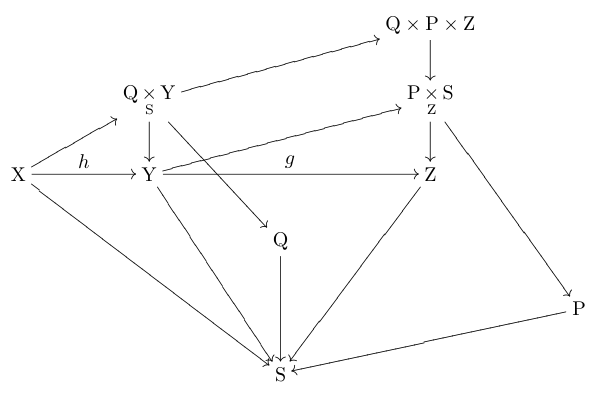
\includegraphics[width=.72\linewidth]{figures/sga4-3/08-gluing-resolutions-p198-composition.png}\end{center}
且 $f=\bar f h$ 经由一个到 $(Q\times_S P)\times_S Z$ 的\Term{quasi-finite}{拟有限}\Term{separated}{分离态射}\Term{resolution}{分解}。
\end{proof}
\SourcePage{199}
Nagata 在 [7] 中断言，任意\Term{noetherian}{诺特}\Term{integral}{整}\Term{separated}{分离}\Term{scheme}{概形}之间的\Term{finite-type}{有限型态射}都是\Term{compactifiable-morphism}{可紧化}的。撰稿人承认未能理解其证明。

现在固定一个\Term{scheme}{概形} $S$，以 $(S)$ 表示 $S$-\Term{scheme}{概形}\Term{category}{范畴}的\Term{subcategory}{子范畴}：\Term{object}{对象}是\Term{quasi-compact}{拟紧}\Term{quasi-separated}{拟分离}的 $S$-\Term{scheme}{概形}，\Term{arrow}{箭头}是 $S$-\Term{compactifiable-morphism}{可紧化}的 $S$-\Term{morphism}{态射}。
\begin{SGAresult}{命题}{3.2.3}
在\Term{category}{范畴} $(S)$ 中：

(i) \Term{open-immersion}{开浸入}（相应地，\Term{proper}{固有态射}）定义一个与 $(S)$ 有相同\Term{object}{对象}的\Term{subcategory}{子范畴} $(S,i)$（相应地，$(S,p)$）。

(ii) $(S,p)$ 中存在\Term{fiber-product}{纤维积}，且它们也是 $(S)$ 中的\Term{fiber-product}{纤维积}。

(iii) 任意\Term{morphism}{态射} $f$ 都是一个\Term{proper}{固有态射} $p$ 与一个\Term{open-immersion}{开浸入}的复合 $f=pj$。
\end{SGAresult}
\begin{proof}
由 3.2.2 (iii)、(iv)、(v)，$(S)$ 中存在\Term{fiber-product}{纤维积}，且也是全体\Term{scheme}{概形}\Term{category}{范畴}中的\Term{fiber-product}{纤维积}。由于两个在 $Y$ 上\Term{proper}{固有}的\Term{scheme}{概形}之\Term{fiber-product}{纤维积} $X=X_1\times_Y X_2$ 仍在 $Y$ 上\Term{proper}{固有}，而一个\Term{scheme}{概形}在 $X$ 上\Term{proper}{固有}当且仅当它在 $X_1,X_2$ 上均\Term{proper}{固有}，条件 (ii) 成立。

若 $f$ 是 $(S)$ 的\Term{morphism}{态射}，依假设它在 $(S)$ 中有\Term{resolution}{分解} $f=pj'$，其中 $p$ \Term{proper}{固有}，$j'$ \Term{quasi-finite}{拟有限}\Term{separated}{分离}。由 EGA IV 18.12.13，$j'$ 有\Term{resolution}{分解} $j'=qj$，其中 $q$ \Term{finite}{有限}，$j$ 是\Term{open-immersion}{开浸入}；又由 3.2.2 (ii)，$q,j$ 属于 $(S)$。于是 $f=(pq)j$，这证明 (iii)。断言 (i) 由 3.2.2 (iii) 得到。
\end{proof}
\textbf{3.2.4.} 本节以下假设给定\Term{category}{范畴} $(S)$ 及其两个\Term{subcategory}{子范畴} $(S,i),(S,p)$，满足
\[
\begin{gathered}
\text{(i) }\operatorname{Ob}(S)=\operatorname{Ob}(S,i)=\operatorname{Ob}(S,p);\\
\text{(ii) }(S,p)\text{ 中存在纤维积，且它们也是 }(S)\text{ 中的纤维积};\\
\text{(iii) }\forall f\in\operatorname{Fl}(S),\ \exists p\in\operatorname{Fl}(S,p),\ \exists j\in\operatorname{Fl}(S,i),\quad f=pj.
\end{gathered}
\]
$(S,i)$ 的\Term{arrow}{箭头}称为\Term{open-immersion}{开浸入}，$(S,p)$ 的\Term{arrow}{箭头}称为\Term{proper}{固有态射}。
\begin{SGAresult}{定义}{3.2.5}
(i) $(S)$ 中\Term{morphism}{态射} $f$（相应地，可\Term{composition-morphism}{复合态射}对 $(f,g)$ 或三元组 $(f,g,h)$）的一个\Term{compactification}{紧化}，是一个\Term{commutative-diagram}{交换图} (3.2.5.1)（相应地，(3.2.5.2) 或 (3.2.5.3)），其水平\Term{arrow}{箭头}为\Term{open-immersion}{开浸入}，斜\Term{arrow}{箭头}为\Term{proper}{固有态射}。

(ii) \Term{compactification}{紧化}之间的\Term{morphism}{态射}，是图 (3.2.5.1)（相应地，等等）之间的\Term{morphism}{态射}，
\SourcePage{200}
它在第一条竖直线上为恒等，在各顶点处均\Term{proper}{固有}。
\begin{center}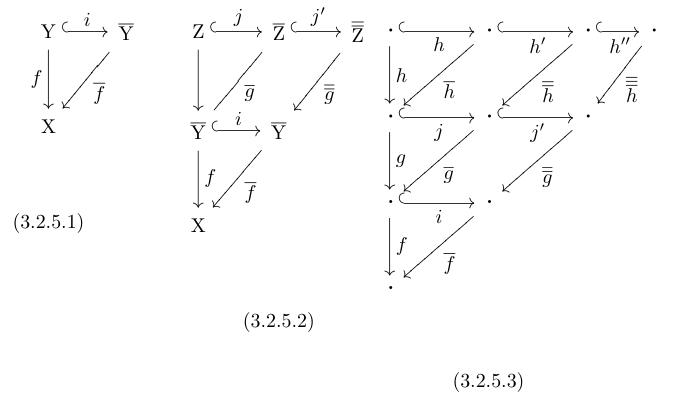
\includegraphics[width=.9\linewidth]{figures/sga4-3/08-gluing-resolutions-p200-compactifications.png}\end{center}
\end{SGAresult}
\begin{SGAresult}{命题}{3.2.6}
(i) 任意\Term{morphism}{态射}（相应地，任意可\Term{composition-morphism}{复合态射}对 $(f,g)$、任意可\Term{composition-morphism}{复合态射}三元组 $(f,g,h)$）都有\Term{compactification}{紧化}。

(ii) $f$ 的\Term{compactification}{紧化}\Term{category}{范畴}是\Term{left-filtered}{左滤过}的。

(iii) 若图 $(3.2.4.2)_i$（$i=1,2$）是 $(f,g)$ 的\Term{compactification}{紧化}，则存在 $(f,g)$ 的\Term{compactification}{紧化} $(3.2.4.2)_3$，以及从它到各 $(3.2.4.2)_i$ 的\Term{compactification}{紧化}\Term{morphism}{态射}。
\end{SGAresult}
\begin{proof}
(i) 一个\Term{morphism}{态射}的情形就是 3.2.4 (iii)。处理三元组的情形：沿用 (3.2.5.3) 的记号，依次构造 $f,g,h$ 的\Term{compactification}{紧化}，然后构造 $ig,jh$ 的\Term{compactification}{紧化}，最后构造 $j'\bar h$ 的\Term{compactification}{紧化}即可。

(ii) 设 $(3.2.5.1)_1,(3.2.5.1)_2$ 是 $f$ 的两个\Term{compactification}{紧化}。$\bar Y_1\times_X\bar Y_2$ 到 $X$ 的\Term{projection}{投影} $\rho$ \Term{proper}{固有}，且 $Y$ 通过 $(i_1,i_2)$ 映入它；由 3.2.4 (iii)，可将此\Term{morphism}{态射}\Term{compactification}{紧化}为 $(i_1,i_2)=qj$。\Term{compactification}{紧化} $f=(\rho\cdot q)j$ \Term{dominant}{支配} $(3.2.4.1)_1,(3.2.4.1)_2$。

若 $r,s$ 是从 $(3.2.4.1)_1$ 到 $(3.2.4.1)_2$ 的两个\Term{morphism}{态射}，则双\Term{arrow}{箭头} $\bar Y_1\rightrightarrows\bar Y_2$ 的核 $K$ 以\Term{proper}{固有态射}映入 $\bar Y_1$，且 $i_1$ 经过 $K$ \Term{resolution}{分解}，记作 $i_1=ki$。若 $i=pi_3$ 是 $i$ 的一个\Term{compactification}{紧化}，则\Term{compactification}{紧化} $f=(\bar f_1kp)i_3$ 的存在表明公理 L2 成立。

(iii) 将\Term{filtered-category}{滤过范畴}的公理 L1 用于由 $(3.2.4.2)_i$（$i=1,2$）得到的 $f,g$ 的\Term{compactification}{紧化}。这样得到 $\bar Y_3,\bar Z_3$，使有\Term{commutative-diagram}{交换图} $(3.2.5.1)_i$（$i=1,2$）：
\SourcePage{201}
\begin{center}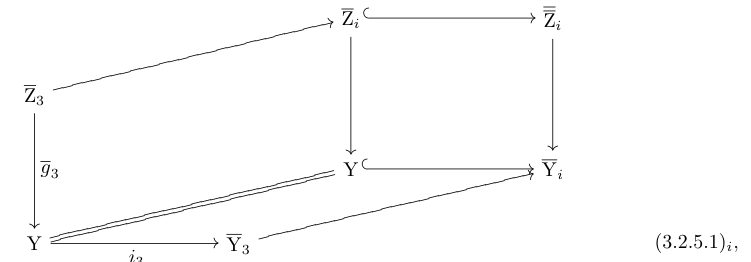
\includegraphics[width=.82\linewidth]{figures/sga4-3/08-gluing-resolutions-p201-cube.png}\end{center}
剩下的是找出 $i_3\bar g_3$ 的一个\Term{compactification}{紧化} $\bar{\bar Z}_3$，使 $\bar{\bar Z}_3$ 能以\Term{proper}{固有态射}映入 $\bar{\bar Z}_i$，形成交换立方图（$i=1,2$）。若 $i_3\bar g_3$ 的\Term{compactification}{紧化}之间某个\Term{morphism}{态射}的靶具有此性质，其源也具有；由 (ii)，只需分别处理 $i=1$ 和 $i=2$。设 $T$ 为 $\bar Y_3$ 与 $\bar{\bar Z}_i$ 在 $\bar Y_i$ 上的\Term{fiber-product}{纤维积}。$T$ 位于一个与所求立方图类似的交换立方图中，惟一的区别是从 $\bar Z_3$ 到 $T$ 的\Term{arrow}{箭头} $k$ 可能不是\Term{open-immersion}{开浸入}。写成 $k=pj$（$p$ \Term{proper}{固有}，$j$ 为\Term{open-immersion}{开浸入}），并用 $p$ 的源 $\bar{\bar Z}_3$ 代替 $T$，就得到所求立方图。
\end{proof}
\textbf{注记 3.2.7。}在\Term{compactifiable-morphism}{可紧化态射}的定义 3.2.1 中，若不要求 $Y$ \Term{quasi-compact}{拟紧}\Term{quasi-separated}{拟分离}，而代之以要求 $j$ 是\Term{quasi-compact}{拟紧}\Term{open-immersion}{开浸入}，不只是\Term{quasi-finite}{拟有限态射}，则命题 3.2.3 仍成立。

\textbf{3.3. \Term{gluing}{粘合}。}回顾，我们假设 3.2.4 的条件成立。

\textbf{3.3.1.} 假设给定：

$\alpha)$ 对每个 $X\in\operatorname{Ob}(S)$，一个\Term{category}{范畴} $F(X)$；

$\beta)$ 一个 $(S,i)$-\Term{cofibered-category}{余纤维范畴} $F_i$ 和一个 $(S,p)$-\Term{cofibered-category}{余纤维范畴} $F_p$；

$\gamma)$ 对每个 $X\in\operatorname{Ob}(S)$，$F(X),(F_i)_X,(F_p)_X$ 之间的\Term{isomorphism}{同构}；

$\delta)$ $F_i$ 的一个\Term{normalization}{正规化}\Term{splitting}{分裂}和 $F_p$ 的一个\Term{normalization}{正规化}\Term{splitting}{分裂}。

由 SGA 1 VI，“\Term{equivalence}{等价}地”可以改为给定 $\alpha)$ 以及：

(i) 对每个\Term{proper}{固有态射} $p:X\to Y$，一个\Term{functor}{函子} $p_*:F(X)\to F(Y)$；

(ii) 对每个可复合的\Term{proper}{固有态射}对 $(p,q)$，一个\Term{functor}{函子}\Term{isomorphism}{同构} $c_{p,q}:p_*q_*\leftrightarrow(pq)_*$；

(i)$'$、(ii)$'$ 对 $(S,i)$ 的相应资料；且这些资料满足：

(a) 若 $p$ 是恒等，则 $p_*,c_{p,q},c_{q,p}$ 都是恒等；
\SourcePage{202}
(b) 对任意可复合的\Term{proper}{固有态射}三元组，有
\[c_{p,qr}\circ(p_* *c_{q,r})=c_{pq,r}\circ(c_{p,q}*r_*);\]
(a)$'$、(b)$'$ 为对 $(S,p)$ 的相应条件。

再假设给定：

(iii) 对每个\Term{commutative-diagram}{交换图} $D$
\[\begin{tikzcd}X\arrow[r,"j'"]\arrow[d,"p'"']&Y\arrow[d,"p"]\\Z\arrow[r,"j"]&T,\end{tikzcd}\qquad j,j'\in\operatorname{Fl}(S,i),\ p,p'\in\operatorname{Fl}(S,p),\]
一个\Term{functor}{函子}\Term{isomorphism}{同构} $d(D):p_*j'_*\leftrightarrow j_*p'_*$。
\begin{SGAresult}{命题}{3.3.2}
若资料 (i)、(ii)、(i$'$)、(ii$'$)、(iii) 满足条件 (a)、(b)、(a$'$)、(b$'$) 及以下的 (c)、(c$'$)，则存在一个且“本质上”惟一的在 $S$ 上的\Term{cofibered-category}{余纤维范畴} $F$，配有与资料 3.3.1 $\gamma)$ 相容的\Term{isomorphism}{同构}
\[F\times_S(S,i)=F_i,\qquad F\times_S(S,p)=F_p,\]
使 (iii) 中的 $d(D)$ 就是\Term{composition-isomorphism}{复合同构}
\[j_*p'_*= (jp')_*=(pj')_*=p_*j'_* .\]
(c) 对任意下列类型的\Term{commutative-diagram}{交换图}，其水平\Term{arrow}{箭头}为\Term{open-immersion}{开浸入}，竖直\Term{arrow}{箭头}为\Term{proper}{固有态射}，
\[\begin{tikzcd}X_1\arrow[r,hook,"i"]\arrow[d,"p_1"']&X_2\arrow[r,hook,"i'"]\arrow[d,"p_2"]&X_3\arrow[d,"p_3"]\\Y_1\arrow[r,hook,"j"]&Y_2\arrow[r,hook,"j'"]&Y_3,\end{tikzcd}\]
由 (iii) 中\Term{isomorphism}{同构} $d$ 构成的下列三角图交换：
\[\begin{tikzcd}p_{3*}i'_*i_*\arrow[rr]\arrow[dr]&&j'_*j_*p_{1*}\\&j'_*p_{2*}i_*\arrow[ur]&.\end{tikzcd}\]
\SourcePage{203}
(c)$'$ 对任意下列类型的\Term{commutative-diagram}{交换图}，其水平\Term{arrow}{箭头}\Term{proper}{固有}，竖直\Term{arrow}{箭头}为\Term{open-immersion}{开浸入}，
\[\begin{tikzcd}X_1\arrow[r,"p"]\arrow[d,hook,"i_1"']&X_2\arrow[r,"p'"]\arrow[d,hook,"i_2"]&X_3\arrow[d,hook,"i_3"]\\Y_1\arrow[r,"q"]&Y_2\arrow[r,"q'"]&Y_3,\end{tikzcd}\]
由 (iii) 中\Term{isomorphism}{同构} $d$ 构成的下列三角图交换：
\[\begin{tikzcd}i_{3*}p'_*p_*\arrow[rr]\arrow[dr]&&q'_*q_*i_{1*}\\&q'_*i_{2*}p_*\arrow[ur]&.\end{tikzcd}\]
\end{SGAresult}
\textbf{3.3.2.1. $f_*$ 的定义。}设 $f:Y\to X$ 是一个\Term{morphism}{态射}。$f$ 的每个\Term{compactification}{紧化}，其图如 (3.2.5 (i))，确定一个从 $F(Y)$ 到 $F(X)$ 的\Term{composite-functor}{复合函子} $\bar f_*i_*$。一个\Term{compactification}{紧化}\Term{morphism}{态射}确定\Term{commutative-diagram}{交换图}
\[\begin{tikzcd}Y\arrow[r,hook,"i_1"]\arrow[d,equal]&\bar Y_1\arrow[d,"p"]\\Y\arrow[r,hook,"i_2"]\arrow[d,"f"']&\bar Y_2\arrow[dl,"\bar f_2"]\\X&\end{tikzcd}\tag{3.3.2.2}\]
故资料 (iii) 给出\Term{isomorphism}{同构}
\[\bar f_{2*}i_{2*}=\bar f_{2*}\circ(i_{2*}\circ1_{Y*})=\bar f_{2*}\circ(p_*\circ i_{1*})=\bar f_{1*}\circ i_{1*}.\]
公理 (c$'$) 还保证：一个\Term{compactification}{紧化}\Term{morphism}{态射}的复合所对应的\Term{isomorphism}{同构}，是各\Term{morphism}{态射}对应\Term{isomorphism}{同构}的复合。由于\Term{compactification}{紧化}\Term{morphism}{态射}\Term{category}{范畴}是\Term{filtered-category}{滤过}的（3.2.6 (ii)），便在 $f$ 的各\Term{compactification}{紧化}所对应的\Term{functor}{函子}间得到一个传递的\Term{isomorphism}{同构}系统。选定其中一个，即定义\Term{functor}{函子} $f_*$。

\textbf{3.3.2.3. 传递\Term{homomorphism}{同态}。}可\Term{composition-morphism}{复合态射}对 $(f,g)$ 的每个\Term{compactification}{紧化}（图 (3.2.5.2)）确定 $f$ 的一个\Term{compactification}{紧化}、$g$ 的一个\Term{compactification}{紧化}、$f\circ g=(\bar f\bar{\bar g})(j'j)$ 的一个\Term{compactification}{紧化}，以及\Term{isomorphism}{同构} $c_{f,g}:(fg)_*\xrightarrow{\sim}f_*g_*$，它是以下\Term{isomorphism}{同构}的复合：
\[(fg)_*=(\bar f\bar{\bar g})_*(j'j)_*=\bar f_*(\bar{\bar g}_*j'_*)j_*=\bar f_*(i_*\bar g_*)j_*=(\bar f_*i_*)(\bar g_*j_*)=f_*g_*\]
（中间的\Term{isomorphism}{同构}来自 (iii)）。
\SourcePage{204}
证明这个\Term{isomorphism}{同构}与 $(f,g)$ 的\Term{compactification}{紧化}的选择无关。由 3.2.6 (iii)，只需比较由两个\Term{compactification}{紧化} $(3.2.4.2)_i$（$i=1,2$）得到的\Term{isomorphism}{同构} $c_{f,g}$，并假设存在从第一个到第二个的\Term{compactification}{紧化}\Term{morphism}{态射}。这些\Term{morphism}{态射}的\Term{arrow}{箭头}用 $p$ 表示。

考虑下列\Term{functor}{函子}\Term{isomorphism}{同构}图。为便于阅读，省去了 $*$：
\begin{center}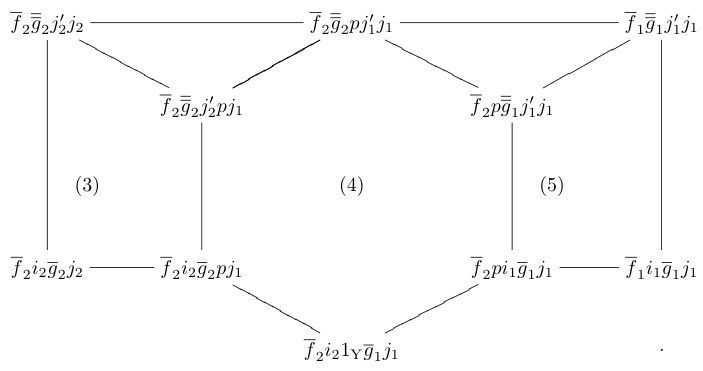
\includegraphics[width=.95\linewidth]{figures/sga4-3/08-gluing-resolutions-p204-comparison.png}\end{center}
a) 第一行的\Term{composition-isomorphism}{复合同构}是 (3.3.2.1) 中 $(fg)_*$ 的两个定义之间的\Term{isomorphism}{同构}。

b) 最后一行的\Term{composition-isomorphism}{复合同构}是 (3.3.2.1) 中 $f_*g_*$ 的两个定义之间的\Term{isomorphism}{同构}。

c) 两端的竖直\Term{isomorphism}{同构}，是由两个\Term{compactification}{紧化}之一得到的 $(fg)_*$ 与 $f_*g_*$ 之间的\Term{isomorphism}{同构} $c_{f,g}$。因此要证明的是整个图的外\Term{boundary}{边界}交换。一个交换的\Term{functor}{函子}图，在将各\Term{functor}{函子}与同一个\Term{functor}{函子}复合后仍然交换。回顾此点，(1) 的交换性由 (c) 应用于下图得到：
\[\begin{tikzcd}Z\arrow[r,hook,"j_1"]\arrow[d,equal]&\bar Z_1\arrow[r,hook,"j'_1"]\arrow[d]&\bar{\bar Z}_1\arrow[d]\\Z\arrow[r,hook,"j_2"]&\bar Z_2\arrow[r,hook,"j'_2"]&\bar{\bar Z}_2.\end{tikzcd}\]
(3)、(5) 的交换性是平凡的；(2) 本质上只涉及\Term{proper}{固有态射}，交换性也是平凡的。还需考察六边形 (4)。
\SourcePage{205}
考虑下列交换立方图：
\begin{center}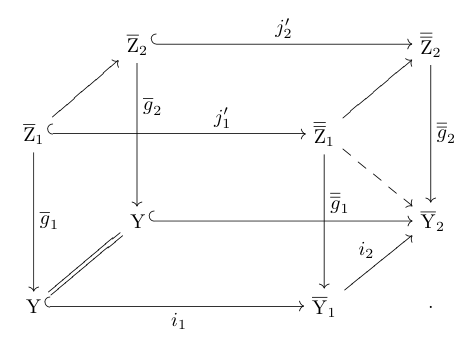
\includegraphics[width=.68\linewidth]{figures/sga4-3/08-gluing-resolutions-p205-cube.png}\end{center}
沿此立方体的棱，从 $\bar Z_1$ 到 $\bar Y_2$ 共有六条路径，每条都与另两条“相邻”；两个相邻路径（即只隔着一个面的路径）对应的\Term{composite-functor}{复合函子}之间有一个\Term{isomorphism}{同构}，而 (4) 的交换性将由这样得到的六边形的交换性推出。

这种图的要旨是：一条棱代表一个\Term{functor}{函子}，一个面代表\Term{composite-functor}{复合函子}之间的\Term{isomorphism}{同构}，一个体代表相容性条件（涉及构成其\Term{boundary}{边界}的各面）。将立方体沿“平面” $\bar Z_1\bar{\bar Z}_1Y\bar Y_2$ \Term{resolution}{分解}为两个三角柱，就可归结为假设 (c$'$)。

确切地说，把该六边形补成以下\Term{isomorphism}{同构}图（仍省略 $*$ 以便阅读）：
\begin{center}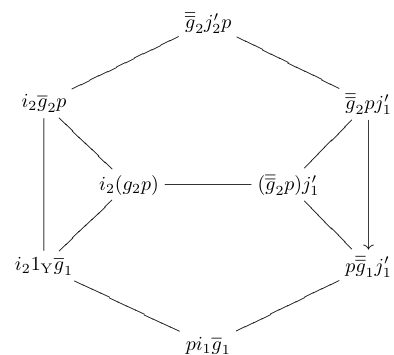
\includegraphics[width=.66\linewidth]{figures/sga4-3/08-gluing-resolutions-p205-hexagon.png}\end{center}
三角图显然交换，两个五边形则由 (c$'$) 交换。
\SourcePage{206}
\textbf{3.3.2.4. \Term{cocycle-condition}{上闭链条件}。}验证 3.3.2.3 所构造的\Term{isomorphism}{同构} $c_{f,g}$，对于任意可\Term{composition-morphism}{复合态射}三元组 $(f,g,h)$ 满足\Term{cocycle-condition}{上闭链条件}。引入 $(f,g,h)$ 的一个\Term{compactification}{紧化}，其图如 (3.2.4.3)，并考虑以下\Term{functor}{函子}\Term{isomorphism}{同构}图：
\begin{center}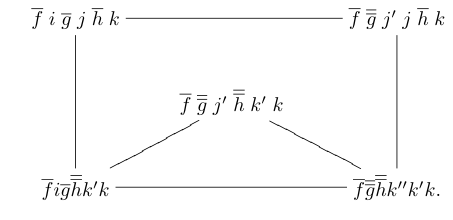
\includegraphics[width=.72\linewidth]{figures/sga4-3/08-gluing-resolutions-p206-cocycle.png}\end{center}
四边形显然交换，两个三角形由 (c)、(c$'$) 交换。整个外\Term{boundary}{边界}的交换性正是要证的结论，因而完成了 3.3.2 的证明。

\textbf{3.3.3.} 假设在 $(S,i),(S,p)$ 上分别给定带有\Term{normalization}{正规化}\Term{splitting}{分裂}的\Term{fibered-category}{纤维范畴} $F_i,F_p$，并假设在每个 $X\in\operatorname{Ob}S$ 处二者有相同的\Term{fiber}{纤维} $F(X)$。

由 SGA 1 VI，“\Term{equivalence}{等价}地”可以改为给定：

(i bis) 对每个\Term{proper}{固有态射} $p:X\to Y$，\Term{functor}{函子} $p^*:F(Y)\to F(X)$；

(ii bis) 对每个可复合的\Term{proper}{固有态射}对 $(p,q)$，\Term{functor}{函子}\Term{isomorphism}{同构} $c_{p,q}:q^*p^*\leftrightarrow(pq)^*$；

(i$'$ bis)、(ii$'$ bis) 对 $(S,i)$ 的相应资料；这些资料满足与 3.3.1 (a)、(b)、(a$'$)、(b$'$) \Term{duality}{对偶}的条件 (a bis)、(b bis)、(a$'$ bis)、(b$'$ bis)。

再假设给定：

(iii bis) 对每个\Term{commutative-diagram}{交换图} $D$
\[\begin{tikzcd}X\arrow[r,"j'"]\arrow[d,"p'"']&Y\arrow[d,"p"]\\Z\arrow[r,"j"]&T,\end{tikzcd}\quad j,j'\in\operatorname{Fl}(S,i),\ p,p'\in\operatorname{Fl}(S,p),\]
\Term{functor}{函子}\Term{isomorphism}{同构} $d(D):j'^*p^*\leftrightarrow p'^*j^*$。

与 3.3.2 (c)、(c$'$) \Term{duality}{对偶}的条件 (c bis)、(c$'$ bis) 留给读者表述。

与上面平行的论证证明下列命题。
\SourcePage{207}
\begin{SGAresult}{命题}{3.3.4}
若资料 (i bis)、(ii bis)、(i$'$ bis)、(ii$'$ bis)、(iii bis) 满足条件 (a bis)、(b bis)、(a$'$ bis)、(b$'$ bis)、(c bis)、(c$'$ bis)，则存在一个且本质上惟一的在 $S$ 上的\Term{cofibered-category}{余纤维范畴} $F$，配有\Term{isomorphism}{同构}
\[F\times_S(S,i)=F_i,\qquad F\times_S(S,p)=F_p,\]
这些\Term{isomorphism}{同构}与等同 $F_{iX}=F_{pX}$（$X\in\operatorname{Ob}S$）相容，并使 (iii bis) 中的\Term{isomorphism}{同构} $d(D)$ 成为\Term{composition-isomorphism}{复合同构}
\[p'^*j^*=(jp')^*=(pj')^*=j'^*p^*.\]
\end{SGAresult}
不过应注意，3.3.4 并不是 3.3.2 的\Term{duality}{对偶}，因为对 $(S,i),(S,p)$ 所作的假设并不\Term{autoduality}{自对偶}。
\SGAsection{4}{解消及其对换基箭头的应用}
\textbf{4.1. \Term{flat-resolution}{平坦解消}。}回顾：若 $f:(X,\mathscr A)\to(Y,\mathscr B)$ 是\Term{ringed-site}{赋环景}（或\Term{ringed-topos}{赋环拓扑斯}）的\Term{morphism}{态射}，则一个左 $\mathscr B$-模\Term{sheaf}{层} $M$ 的\Term{inverse-image}{逆像}是左 $\mathscr A$-模\Term{sheaf}{层} $\mathscr A\otimes_{f^*\mathscr B}f^*M$。
\begin{SGAresult}{命题}{4.1.1}
设 $f:(X,\mathscr A)\to(Y,\mathscr B)$ 是\Term{ringed-site}{赋环景}\Term{morphism}{态射}，$K$ 是右 $\mathscr A$-模\Term{sheaf}{层}，$0\to L\to M\to N\to0$ 是左 $\mathscr B$-模\Term{sheaf}{层}的\Term{exact-sequence}{正合列}。若 $M,N$ \Term{flat}{平坦}，则

(i) $L$ \Term{flat}{平坦}；

(ii) 下列为\Term{exact-sequence}{正合列}：
\[0\longrightarrow K\otimes_{\mathscr A}f^*L\longrightarrow K\otimes_{\mathscr A}f^*M\longrightarrow K\otimes_{\mathscr A}f^*N\longrightarrow0.\]
\end{SGAresult}
\begin{proof}
将 $f$ \Term{resolution}{分解}为\Term{arrow}{箭头} $(X,\mathscr A)\xrightarrow{u}(X,f^*\mathscr B)\xrightarrow{v}(Y,\mathscr B)$。\Term{functor}{函子} $v^*$ \Term{exact}{正合}，且把\Term{flat}{平坦}模变为\Term{flat}{平坦}模（IV 15），故只须对 $u$ 证明 4.1.1。\Term{isomorphism}{同构}
\[K\otimes_{\mathscr A}(\mathscr A\otimes_{f^*\mathscr B}P)=K\otimes_{f^*\mathscr B}P\tag{4.1.1.1}\]
又将我们归结为 $f$ 为恒等的情形。
\SourcePage{208}
取\Term{exact-sequence}{正合列} $0\to R\to P\to K\to0$，其中 $P$ \Term{flat}{平坦}（4.1.2）。下图的行与列均\Term{exact}{正合}：
\[\begin{tikzcd}& &0\arrow[d]&&\\&R\otimes L\arrow[r]\arrow[d]&P\otimes L\arrow[r]\arrow[d]&K\otimes L\arrow[r]\arrow[d]&0\\0\arrow[r]&R\otimes M\arrow[r]\arrow[d]&P\otimes M\arrow[r]\arrow[d]&K\otimes M\arrow[r]\arrow[d]&0\\0\arrow[r]&R\otimes N\arrow[r]\arrow[d]&P\otimes N\arrow[r]\arrow[d]&K\otimes M\arrow[r]\arrow[d]&0\\&0&0&0&.\end{tikzcd}\]
对前两列应用蛇形图，得到
\[0\xrightarrow{j}K\otimes L\longrightarrow K\otimes M,\]
故 (ii) 成立。现在不再假设 $P$ \Term{flat}{平坦}，则已知上图三列及两行都是短\Term{exact-sequence}{正合列}；故第一行\Term{exact}{正合}，即 $L$ \Term{flat}{平坦}。
\end{proof}
\textbf{4.1.2.} 设 $\mathscr S$ 是\Term{ringed-site}{赋环景}\Term{category}{范畴}的一个\Term{subcategory}{子范畴}。$\mathscr S$ 中各\Term{ringed-site}{赋环景}上的模\Term{sheaf}{层}构成\Term{category}{范畴} $\mathscr M$，它在 $\mathscr S$ 上是阿贝尔的（2.2.2），且既\Term{fibered-category}{纤维}又\Term{cofibered-category}{余纤维}；它的\Term{fiber}{纤维}是通常的景上模\Term{sheaf}{层}\Term{category}{范畴}的\Term{opposite-category}{反范畴}。以 $K(\mathscr S)$ 表示\Term{category}{范畴} $K(\mathscr M)$（2.2.8），以 $K^+(\mathscr S)$（相应地 $K^-(\mathscr S)$）表示其\Term{full-subcategory}{满子范畴}，\Term{fibre-category}{纤维范畴}为各 $S\in\operatorname{Ob}\mathscr S$ 对应的 $K^+(S)$（相应地 $K^-(S)$）的\Term{opposite-category}{反范畴}。\Term{category}{范畴} $K(\mathscr S),K^+(\mathscr S),K^-(\mathscr S)$ 在 $\mathscr S$ 上三角化，且既\Term{fibered-category}{纤维}又\Term{cofibered-category}{余纤维}。

设 $f:S\to S'$ 是 $\mathscr S$ 的一个\Term{arrow}{箭头}。每个\Term{injective-object}{内射对象}对\Term{functor}{函子} $Rf_*$ \Term{acyclic}{无环}（1.2.3），每个\Term{flat}{平坦}模\Term{sheaf}{层}对\Term{functor}{函子} $Lf^*$ \Term{acyclic}{无环}（4.1.1 与 1.2.6），故有\Term{derived-functor}{导出函子}（1.2.7）
\[Rf_*:D^+(S)\longrightarrow D^+(S')\tag{4.1.2.1}\]
\[Lf^*:D^-(S)\longrightarrow D^-(S').\tag{4.1.2.2}\]
若 $Rf_*$（相应地 $Lf^*$）\Term{dimension}{维数}\Term{finite}{有限}，则在 (4.1.2.1)（相应地 (4.1.2.2)）中，可以把上标 $+$（相应地 $-$）换成 $b$、$-$（相应地 $+$），或将它去掉（1.2.10）。

以 $D(\mathscr S)$（相应地 $D^+(\mathscr S),D^-(\mathscr S)$）表示从 $K(\mathscr S)$（相应地 $K^+(\mathscr S),K^-(\mathscr S)$）通过反演\Term{quasi-isomorphism}{拟同构}得到的\Term{category}{范畴}。
\begin{SGAresult}{评注}{4.1.3}
（“\Term{trivial-duality}{平凡对偶}定理”。）
\SourcePage{209}
(a) 假设所有\Term{functor}{函子} $Rf_*$（相应地 $Lf^*$）均为\Term{finite}{有限}维。则：

(i) $D(\mathscr S)$ 的形成与任意\Term{base-category}{基范畴}变换 $\mathscr S'\to\mathscr S$ 可交换。\Term{category}{范畴} $D(\mathscr S)$ 在 $\mathscr S$ 上三角化（2.2.3），其\Term{fiber}{纤维}可等同于各 $S\in\operatorname{Ob}\mathscr S$ 对应的\Term{category}{范畴} $D(S)$ 的\Term{opposite-category}{反范畴}。

(ii) \Term{category}{范畴} $D(\mathscr S)$ 在 $\mathscr S$ 上是\Term{cofibered-category}{余纤维}的（相应地，\Term{fibered-category}{纤维}的）。设 $f:S\to S'$；若 $Lf^*$（相应地 $Rf_*$）\Term{finite}{有限}维，则每个 $D(S')$（相应地 $D(S)$）中的\Term{object}{对象}，都有相对于 $\mathscr S$ 上\Term{category}{范畴} $D(\mathscr S)$ 的沿 $f$ 的\Term{inverse-image}{逆像}（相应地\Term{direct-image}{直接像}）。相应的\Term{inverse-image}{逆像}和\Term{direct-image}{直接像}\Term{functor}{函子}等同于 $Lf^*,Rf_*$。

(iii) $D^-(S')$（相应地 $D^+(S)$）中的每个\Term{object}{对象}，都有在 $D(\mathscr S)$ 意义下的\Term{inverse-image}{逆像}（相应地\Term{direct-image}{直接像}），该\Term{functor}{函子}等同于 $Lf^*$（相应地 $Rf_*$）。

(b) (i) $D^-(\mathscr S)$（相应地 $D^+(\mathscr S)$）的形成与任意\Term{base-category}{基范畴}变换 $\mathscr S'\to\mathscr S$ 可交换。该\Term{category}{范畴}在 $\mathscr S$ 上三角化，其\Term{fiber}{纤维}等同于各 $D^-(S)$（相应地 $D^+(S)$）的\Term{opposite-category}{反范畴}。

(ii) \Term{category}{范畴} $D^-(\mathscr S)$（相应地 $D^+(\mathscr S)$）在 $\mathscr S$ 上是\Term{fibered-category}{纤维}的（相应地\Term{cofibered-category}{余纤维}的）；“\Term{inverse-image}{逆像}”（相应地“\Term{direct-image}{直接像}”）\Term{functor}{函子}等同于\Term{derived-functor}{导出函子} $Lf^*$（相应地 $Rf_*$）。

(iii) 若 $f:S\to S'$ 使 $Rf_*$（相应地 $Lf^*$）\Term{finite}{有限}维，则 $D^-(S)$（相应地 $D^+(S')$）中的任意\Term{object}{对象}都有 $D^-(\mathscr S)$ 意义下的\Term{direct-image}{直接像}（相应地 $D^+(\mathscr S)$ 意义下的\Term{inverse-image}{逆像}），且该\Term{functor}{函子}等同于 $Rf_*$（相应地 $Lf^*$）。
\end{SGAresult}
\begin{proof}
只需验证在每种情形中 2.4.1 或 2.4.3 的假设满足，其余断言在\Term{base-change}{基变换} $\{S\}\to\mathscr S$ 或 $I\to\mathscr S$ 后由 2.3.5、1.2.10 得出。在 (b) 中，\Term{flat}{平坦}\Term{sheaf}{层}（相应地\Term{flasque-sheaf}{松弛层}）组成的\Term{complex}{复形}满足 2.4.1 的假设。在 (a) 中，应用 2.4.3，使我们只需考虑那些 $Rf_*$（相应地 $Lf^*$）的\Term{dimension}{维数}受一个固定 $N$ 控制的 $f$。证明存在“足够多”的\Term{complex}{复形} $K$，其各\Term{set-component}{分量}的所有\Term{direct-image}{直接像}（相应地\Term{inverse-image}{逆像}）对于所考虑的\Term{direct-image}{直接像}（相应地\Term{inverse-image}{逆像}）\Term{functor}{函子}均\Term{acyclic}{无环}。设 $K$ 为一\Term{complex}{复形}，$K^*$（相应地 $K_*$）为由各\Term{set-component}{分量}\Term{flasque-sheaf}{松弛}（相应地\Term{flat}{平坦}）的\Term{complex}{复形}组成的 Cartan--Eilenberg \Term{resolution}{解消}。若 $n>N$，则
\[f_*\tau''_{<n}(K^*)=\tau''_{<n}f_*(K^*)\quad\bigl(\text{相应地 }f^*\tau''_{>-n}(K_*)=\tau''_{>-n}f^*(K_*)\bigr),\]
其中 $\tau''$ 表示对第二个\Term{differential}{微分}的\Term{truncation}{截断}。对于 $n>2N$，由此得出 $\tau''_{<n}(K^*)$（相应地 $\tau''_{>-n}(K_*)$）满足 2.4.3 的假设，而任意\Term{complex}{复形} $K$ 都是一个以此类\Term{complex}{复形}为靶（相应地为源）的\Term{quasi-isomorphism}{拟同构}的源（相应地靶）。
\end{proof}
\SourcePage{210}
\textbf{4.1.4.} 考虑\Term{ringed-site}{赋环景}的\Term{commutative-square}{交换方块}（参见 0.11）
\[\begin{tikzcd}X'\arrow[r,"g'"]\arrow[d,"f'"']&X\arrow[d,"f"]\\S'\arrow[r,"g"]&S.\end{tikzcd}\tag{4.1.4.1}\]
可考虑\Term{site}{景}\Term{category}{范畴}中只含此图的\Term{subcategory}{子范畴}；当 4.1.3 适用时，用 2.1.2 定义从 $Lg^*Rf_*$ 到 $Rf'_*Lg'^*$ 的“\Term{base-change}{换基}\Term{morphism}{态射}”。
\begin{SGAresult}{命题}{4.1.5}
2.1.2 中从 $Lg^*Rf_*$ 到 $Rf'_*Lg'^*$ 的\Term{base-change}{换基}\Term{arrow}{箭头}，在下列各种情形中均有定义：

(i) 在\Term{category}{范畴} $D^+$ 中工作，且 $Lg^*,Lg'^*$ \Term{finite}{有限}维。

(ii) 在\Term{category}{范畴} $D^-$ 中工作，且 $Rf_*,Rf'_*$ \Term{finite}{有限}维。

(iii) 在整个\Term{derived-category}{导出范畴}中工作，且 $Rf_*,Rf'_*,Lg^*,Lg'^*$ \Term{finite}{有限}维，并且 $Lf^*,Lf'^*$ 亦\Term{finite}{有限}维（或者 $Rg_*,Rg'_*$ 亦\Term{finite}{有限}维）。
\end{SGAresult}
注意 (iii) 的最后一个假设似乎颇为荒诞。除非所考虑的\Term{site}{景}有\Term{enough-points}{足够多的点}（4.2.12），撰稿人不知道如何去掉它。这个\Term{base-change}{换基}\Term{arrow}{箭头}的\Term{functorial}{函子性}质由描述 2.1.2 立即得到。

\textbf{4.1.6.} 设 $(S,\mathscr A)$ 是\Term{ringed-site}{赋环景}，考虑“\Term{tensor-product}{张量积}”\Term{functor}{函子}
\[\otimes:\operatorname{Mod}_d(S,\mathscr A^\circ)\times\operatorname{Mod}_g(S,\mathscr A)\longrightarrow\operatorname{Mod}(S,\mathscr C),\]
其中 $\mathscr C$ 是 $\mathscr A$ 的\Term{center}{中心}。采用 1.1.6 的方法，在应用时用\Term{direct-sum}{直和}定义\Term{double-complex}{双复形}所对应的\Term{simple-complex}{单复形}，可以把该\Term{functor}{函子}扩展为仍记作 $\otimes$ 的\Term{functor}{函子}
\[\otimes:K(S,\mathscr A^\circ)\times K(S,\mathscr A)\longrightarrow K(S,\mathscr C).\]
\begin{SGAresult}{命题}{4.1.7}
沿用以上记号：

(i) \Term{tensor-product}{张量积}\Term{functor}{函子}可左\Term{derive}{导出}（1.2.1），得到“全\Term{tensor-product}{张量积}”\Term{functor}{函子}
\[\mathbin{\otimes^{\mathbf L}}:D^-(S,\mathscr A^\circ)\times D^-(S,\mathscr A)\longrightarrow D^-(S,\mathscr C);\]
(ii) 对于\Term{bounded-above}{上有界}的\Term{complex}{复形}对 $(K,L)$，只要 $K$ 或 $L$ 的\Term{set-component}{分量}\Term{flat}{平坦}，它便对 $\otimes^{\mathbf L}$ \Term{derived-adapted}{适配}。
\end{SGAresult}
证明是标准的。
\SourcePage{211}
\textbf{记号 4.1.8。}若 $K\in D^-(S,\mathscr A^\circ),L\in D^-(S,\mathscr A)$，以 $K\otimes^{\mathbf L}L$ 表示其全\Term{tensor-product}{张量积}。\Term{sheaf}{层}
\[H_k(K\otimes^{\mathbf L}L)=H^{-k}(K\otimes^{\mathbf L}L)\]
记作 $\operatorname{Tor}_k(K,L)$，称为 $K,L$ 的第 $k$ 个\Term{local-scheme}{局部}超 Tor。

设 $K\in D^-(S,\mathscr A^\circ),L\in D^-(S,\mathscr A)$。若 $i>k$ 时 $H^i(K)=0$，$i>\ell$ 时 $H^i(L)=0$，则可验证，$i>k+\ell$ 时 $H^i(K\otimes^{\mathbf L}L)=0$，且
\[H^{k+\ell}(K\otimes^{\mathbf L}L)=H^k(K)\otimes H^\ell(L).\]
固定 $K$，把 $K\otimes^{\mathbf L}L$ 看作关于 $L$ 的\Term{functor}{函子}。若采用 1.2.9 中将\Term{cohomological-amplitude}{上同调振幅}定义为 $\mathbf Z$ 中区间的定义，则该区间的上界是平凡的：它是使 $H^i(K)\ne0$ 的最大整数 $i$。下界则更为有趣：
\begin{SGAresult}{定义}{4.1.9}
\Term{complex}{复形} $K\in\operatorname{Ob}D^b(S,\mathscr A^\circ)$ 称为\Term{tor-dimension}{Tor 维数} $\le n$，若下列\Term{equivalence}{等价}条件成立：

(i) 对任意 $\mathscr A$-模 $L$，$k>n$ 时 $\operatorname{Tor}_k(K,L)=0$。

(ii) 对任意满足 $i<\ell$ 时 $H^i(L)=0$ 的 $\mathscr A$-模\Term{complex}{复形} $L$，$i<\ell-n$ 时 $H^i(K\otimes^{\mathbf L}L)=0$。

(iii) 存在以 $K$ 为靶的\Term{quasi-isomorphism}{拟同构}，其源 $K'$ 是\Term{set-component}{分量}\Term{flat}{平坦}、且在 $i<-n$ 时为零的\Term{complex}{复形}。
\end{SGAresult}
\textbf{4.1.10.} 还可以作以下变式：

(i) 若 $K\in\operatorname{Ob}D^b(S,\mathscr A^\circ)$ 有\Term{finite}{有限}\Term{tor-dimension}{Tor 维数}，且 $L\in\operatorname{Ob}D(S,\mathscr A)$，则\Term{functor}{函子} $\otimes^{\mathbf L}$ 在 $(K,L)$ 处有定义（1.2.1）。

(ii) 若 $K\in\operatorname{Ob}K^b(S,\mathscr A^\circ)$ 的各\Term{set-component}{分量}有\Term{finite}{有限}\Term{tor-dimension}{Tor 维数}，则\Term{functor}{函子} $L\mapsto K\otimes L$（$L\in K(S,\mathscr A)$）可左\Term{derive}{导出}。

(iii) 若每个模都有\Term{finite}{有限}\Term{tor-dimension}{Tor 维数}，则\Term{functor}{函子} $\otimes$ \Term{derivable-category}{可导出}为
\[\mathbin{\otimes^{\mathbf L}}:D(S,\mathscr A^\circ)\times D(S,\mathscr A)\longrightarrow D(S,\mathscr C).\]

\textbf{4.2. Godement \Term{flasque-resolution}{松弛解消}。}
\textbf{4.2.1.} 设 $S$ 为\Term{topos}{拓扑斯}，$X$ 为\Term{set}{集合}。给定以 $X$ 为指标的 $S$ 的点族，\Term{equivalence}{等价}于给定从\Term{discrete-topology}{离散拓扑}\Term{space}{空间} $X$ 所定义的\Term{topos}{拓扑斯}到 $S$ 的\Term{morphism}{态射} $k:\operatorname{Top}(X)\to S$。此点族为\Term{conservative}{保守}的（IV 6.4.1），当且仅当对 $S$ 的任意\Term{sheaf}{层} $F$，\Term{adjoint}{伴随箭头} $F\to k_*k^*F$ 为\Term{monomorphism}{单态射}（参见 IV 6.4.0）。
\begin{SGAresult}{定义}{4.2.2}
设 $k:\operatorname{Top}(X)\to S$ 是\Term{topos}{拓扑斯} $S$ 的\Term{conservative}{保守}点族。$S$ 的阿贝尔\Term{sheaf}{层} $F$ 的 \Term{godement-resolution}{Godement 解消}或（相对于 $X$ 的）\Term{canonical}{典范}\Term{flasque-resolution}{松弛解消}，记作 $C_X^*(F)$（或简写 $C^*(F)$），是 $F$ 的如下右\Term{resolution}{解消}：

1) $C^0(F)=k_*k^*F$，$\varepsilon:F\to C^0(F)$ 为\Term{adjoint}{伴随箭头}。
\SourcePage{212}
2) 令 $d^{-1}=\varepsilon$；对 $n\ge0$ 递归定义
\[C^{n+1}(F)=C^0(\operatorname{coker}d^{n-1}),\]
而 $d^n$ 定义为复合\Term{arrow}{箭头}
\[d^n:C^n(F)\longrightarrow\operatorname{coker}(d^{n-1})\longrightarrow C^0(\operatorname{coker}(d^{n-1})).\]
\end{SGAresult}
\begin{SGAresult}{命题}{4.2.3}
在 4.2.2 的假设下：

(i) $C(F)$ 是\Term{flasque-sheaf}{松弛层}（V 3.7）。

(ii) $C^n(F)$ 是关于 $F$ 的\Term{exact-functor}{正合函子}。

(iii) \Term{complex}{复形} $C^*(F)$ 在点 $x\in X$ 的\Term{fiber}{纤维}是 $F_x$ 的一个\Term{canonical}{典范}\Term{splitting}{分裂}的\Term{resolution}{解消}。
\end{SGAresult}
\begin{proof}
$C^n(F)$ 是\Term{discrete-topology}{离散拓扑}\Term{space}{空间} $X$ 上的\Term{sheaf}{层}（自动\Term{flasque-sheaf}{松弛}）的\Term{direct-image}{直接像}，因而\Term{flasque-sheaf}{松弛}。

\Term{functor}{函子} $k^*,k_*$ \Term{exact}{正合}，故 $C^0$ \Term{exact}{正合}。对 $n\ge0$ 归纳证明\Term{functor}{函子} $Z^n(F)=\operatorname{coker}(d^{n-1})$ \Term{exact}{正合}，从而 $C^{n+1}=C^0Z^n$ 也\Term{exact}{正合}。令 $Z^{-1}(F)=F$。\Term{sheaf}{层}的\Term{exact-sequence}{正合列} $0\to F'\to F\to F''\to0$，对 $n\ge0$ 给出图
\[\begin{tikzcd}&0\arrow[d]&0\arrow[d]&0\arrow[d]&\\0\arrow[r]&Z^{n-1}(F')\arrow[r]\arrow[d]&Z^{n-1}(F)\arrow[r]\arrow[d]&Z^{n-1}(F'')\arrow[r]\arrow[d]&0\\0\arrow[r]&C^n(F')\arrow[r]\arrow[d]&C^n(F)\arrow[r]\arrow[d]&C^n(F'')\arrow[r]\arrow[d]&0\\0\arrow[r]&Z^n(F')\arrow[r]\arrow[d]&Z^n(F)\arrow[r]\arrow[d]&Z^n(F'')\arrow[r]\arrow[d]&0\\&0&0&0&.\end{tikzcd}\]
其列均\Term{exact}{正合}，由归纳假设，前两行也\Term{exact}{正合}。故第三行\Term{exact}{正合}，(ii) 得证。

短\Term{exact-sequence}{正合列}
\[0\longrightarrow Z^{n+1}(F)\longrightarrow C^n(F)\longrightarrow Z^n(F)\longrightarrow0\]
都是短\Term{exact-sequence}{正合列}
\[0\longrightarrow F\xrightarrow{\varepsilon}C^0(F)\longrightarrow Z^0(F)\longrightarrow0\tag{4.2.3.1}\]
的特例（将 $F$ 换为 $Z^{n-1}(F)$）。为证明 (iii)，只需证明此列沿 $k$ 的\Term{inverse-image}{逆像}\Term{canonical}{典范}\Term{splitting}{分裂}。
\SourcePage{213}
确实，复合\Term{arrow}{箭头}
\[k^*F\xrightarrow{k^*(\varepsilon)}k^*C^0F=k^*(k_*k^*)F=(k^*k_*)k^*F\longrightarrow k^*F\]
是恒等。
\end{proof}
\textbf{注记 4.2.4。}若 $(x_i)_{i\in X}$ 是一个\Term{site}{景}的\Term{conservative}{保守}点族，它对应于所生成\Term{topos}{拓扑斯}的一个\Term{conservative}{保守}点族，因此仍可定义\Term{canonical}{典范}\Term{flasque-resolution}{松弛解消}。

\textbf{注记 4.2.5。}若 $S$ 是\Term{ringed-topos}{赋环拓扑斯}，则\Term{functor}{函子} $C^n$ 将模变为模。

\textbf{注记 4.2.6。}设 $\mathscr S$ 为一个由\Term{site}{景}组成的\Term{category}{范畴}。假设对每个 $S\in\operatorname{Ob}\mathscr S$ 给定一个\Term{set}{集合} $S_d$，及以 $S_d$ 为指标的 $S$ 的\Term{conservative}{保守}点族 $k_S:\operatorname{Top}(S_d)\to S$。假设 $S_d$ 关于 $S$ 是\Term{functorial}{函子性}的，且下图交换：
\[\begin{tikzcd}\operatorname{Top}(S_d)\arrow[r,"f_d"]\arrow[d,"k_S"']&\operatorname{Top}(T_d)\arrow[d,"k_T"]\\S\arrow[r,"f"]&T.\end{tikzcd}\]
则对应的\Term{canonical}{典范}\Term{flasque-resolution}{松弛解消}“关于 $S$ 是\Term{functorial}{函子性}的”。

若 $\mathscr S$ 为\Term{topological-space}{拓扑空间}\Term{category}{范畴}，可取 $S_d$ 为\Term{underlying-set}{底集}。

若 $\mathscr S$ 是一个\Term{scheme}{概形} $S_0$ 上\Term{local-scheme}{局部}\Term{finite-type}{有限型}\Term{scheme}{概形} $S$ 的\Term{etale}{平展}\Term{site}{景}所成的\Term{category}{范畴}，并且对每个 $s\in S_0$，$\overline{k(s)}$ 是 $k(s)$ 的\Term{algebraic-closure}{代数闭包}，则可取 $S_d$ 为 $S$ 中取值于某个 $\overline{k(s)}$ 的点所成的\Term{set}{集合}。

若把\Term{algebraic-closure}{代数闭包} $\overline{k(s)}$ 换成\Term{large-relative-to-cardinal}{足够大}的\Term{algebraically-closed}{代数闭}\Term{group-extension}{扩张}，则可把“\Term{finite-type}{有限型}”条件换成一个\Term{cardinal}{基数}条件。

\textbf{4.2.7.} \Term{canonical}{典范}\Term{flasque-resolution}{松弛解消}的用途之一，是可以构造同时对“\Term{tensor-product}{张量积}”型\Term{functor}{函子}和“\Term{direct-image}{直接像}”型\Term{functor}{函子}\Term{derived-adapted}{适配}的\Term{complex}{复形}。借此可以给出一种也许更容易理解的\Term{base-change}{换基}\Term{morphism}{态射}构造（4.1.5）。
\begin{SGAresult}{引理}{4.2.8}
设 $f:(S,\mathscr A)\to(S',\mathscr B)$ 为\Term{ringed-site}{赋环景}\Term{morphism}{态射}，$K\in\operatorname{Ob}K(S,\mathscr A^\circ),L\in\operatorname{Ob}K(S',\mathscr B)$ 为\Term{complex}{复形}，$k:\operatorname{Top}(X)\to S$ 为 $S$ 的\Term{conservative}{保守}点集。假设下列条件之一成立：

(a) $K,L$ 的\Term{cohomology}{上同调}\Term{bounded-above}{上有界}；

(b) $\mathscr A$ 在 $f^*\mathscr B$ 上有\Term{finite}{有限}\Term{tor-dimension}{Tor 维数}，且 $K\in\operatorname{Ob}D^b(S,\mathscr A^\circ)$ 有\Term{finite}{有限}\Term{tor-dimension}{Tor 维数}；
\SourcePage{214}
(c) $L\in\operatorname{Ob}D^b(S',\mathscr B)$ 有\Term{finite}{有限}\Term{tor-dimension}{Tor 维数}。

则\Term{functor}{函子} $(K,L)\mapsto K\otimes f^*L$ 在 $(K,L)$ 处\Term{derivable-category}{可导出}（1.2.1），以 $\otimes^{\mathbf L}Lf^*$ 表示其\Term{derive}{导出}。

(i) 若 $x$ 是 $S$ 的一点，则
\[(K\otimes^{\mathbf L}Lf^*L)_x\simeq K_x\otimes^{\mathbf L}_{\mathscr B_{f(x)}}L_{f(x)}.\]
(ii) 对 $(K,L)$ 而言，关于 $\otimes^{\mathbf L}f^*$ 左\Term{derived-adapted}{适配}（1.2.1），当且仅当对所有 $x\in X$，$(K_x,L_{f(x)})$ 关于\Term{functor}{函子} $\otimes_{\mathscr B_{f(x)}}$ 左\Term{derived-adapted}{适配}。

(iii) 在假设 (a) 或 (b) 下，关于 $L$ 的\Term{functor}{函子} $K\otimes^{\mathbf L}f^*L$ 的\Term{cohomological-amplitude}{上同调振幅}包含于 $d$（1.2.9），当且仅当对所有 $x\in V$，$\mathscr B_{f(x)}$-模\Term{complex}{复形} $K_x$ 的 Tor 振幅包含于 $d$。
\end{SGAresult}
此引理的证明是标准的；它表达所考虑\Term{functor}{函子}的“逐点性质”。

\textbf{4.2.9.} 设 $L$ 是\Term{complex}{复形}。$L$ 的（相对于 $X$ 的）\Term{godement-resolution}{Godement 解消}，指\Term{double-complex}{双复形} $C^*L$ 所对应的\Term{simple-complex}{单复形}（用\Term{direct-sum}{直和}定义）（1.1.4）。$n$ 阶\Term{truncation}{截断}的\Term{godement-resolution}{Godement 解消} $\tau''_{\le n}C^*L$，指由 $C^*L$ 沿 Godement \Term{differential}{微分}方向\Term{truncation}{截断}（1.1.15）得到的\Term{double-complex}{双复形}所对应的\Term{simple-complex}{单复形}。由 4.2.3 (iii)，在 $X$ 的每个点处，$L$ 与\Term{complex}{复形} $\tau''_{\le n}C^*L,C^*L$ \Term{homotopy}{同伦}；因而这些\Term{complex}{复形}对于“\Term{tensor-product}{张量积}”型\Term{functor}{函子}而言“与 $L$ 一样好”（4.2.8）。
\begin{SGAresult}{命题}{4.2.10}
设 $(S,\mathscr A)$ 是\Term{ringed-site}{赋环景}，$X$ 是 $S$ 的\Term{conservative}{保守}点集，$N,M\in\mathbf N\cup\{\infty\}$，且 $N$ 或 $M<\infty$。设 $A$ 是 $K(S)$ 中由满足下列条件的\Term{complex}{复形} $L$ 构成的\Term{subcategory}{子范畴}：

(a) 若 $N=\infty$，则 $i$ 充分大时 $H^i(L)=0$；若 $M=\infty$，则 $i$ 充分小时 $H^i(L)=0$。

(b) 对任意 $x\in X$ 及\Term{tor-dimension}{Tor 维数} $\le N$ 的 $\mathscr A_x$-模 $Q$，\Term{complex}{复形} $L_x$ 对\Term{functor}{函子} $M_x\otimes_{\mathscr A_x}*$ 左\Term{derived-adapted}{适配}。

(c) 对任意\Term{cohomological-dimension}{上同调维数} $\le M$ 的\Term{topos}{拓扑斯}\Term{morphism}{态射} $f:X^\sim\to E$，\Term{complex}{复形} $L$ 对\Term{functor}{函子} $f_*$ 右\Term{derived-adapted}{适配}。

则 $A\hookrightarrow K(S)$ 诱导如下\Term{category}{范畴}之间的\Term{equivalence}{等价}：在 $A$ 中反演\Term{quasi-isomorphism}{拟同构}得到的\Term{category}{范畴}，与\Term{category}{范畴} $D^*(S)$。这里，$N<M=\infty$ 时 $*=+$，$M<N=\infty$ 时 $*=-$，$N,M<\infty$ 时无上标。
\end{SGAresult}
\begin{proof}
设 $K$ 满足 (a)。若 $N=\infty$，则 $i$ 充分大时\Term{canonical}{典范}\Term{arrow}{箭头} $a:K_1=\sigma_{\le i}K\to K$ 是\Term{quasi-isomorphism}{拟同构}。若 $N<\infty$，令 $K_1=K$。取 $K_1$ 的\Term{flat}{平坦} Cartan--Eilenberg \Term{resolution}{解消} $K_1^*$，并令 $K_2=\tau''_{\ge N}K_1^*$（沿新\Term{differential}{微分}方向\Term{truncation}{截断}）。从 $K_2$ 到 $K$ 的复合\Term{arrow}{箭头}为\Term{quasi-isomorphism}{拟同构}，且 $K_2$ 满足 (b)。

设 $K$ 满足 (a)、(b)。若 $M=\infty$，则 $N<\infty$；对充分大的 $i$，$b:K\to\sigma_{\ge i}K_1=K_3$ 是\Term{quasi-isomorphism}{拟同构}，且 $K_3$ 仍满足 (a)、(b)。
\SourcePage{215}
若 $M<\infty$，令 $K=K_3$。设 $K_4=\sigma''_{\le M}C^*K_3$。则 $K_4$ 满足 (a)、(c)，并由 4.2.3 (iii) 满足 (b)。

因此\Term{continuous}{连续}两次应用 [CD I 2.4.2]，即得命题。
\end{proof}
\textbf{变式 4.2.11。}若 $N<\infty$（相应地 $M<\infty$，或 $N,M<\infty$），也可同样在\Term{bounded-below}{下有界}（相应地\Term{bounded-above}{上有界}，或\Term{bounded}{有界}）\Term{complex}{复形}中工作。

\textbf{4.2.12.} 当所考虑的\Term{site}{景}有\Term{enough-points}{足够多的点}时，以下说明怎样用这些构造，在比 4.1.4 更一般的假设下定义那里的\Term{base-change}{换基}\Term{morphism}{态射}。

设有\Term{site}{景}的\Term{commutative-diagram}{交换图}（参见 0.11）
\[\begin{tikzcd}X'\arrow[r,"g'"]\arrow[d,"f'"']&X\arrow[d,"f"]\\S'\arrow[r,"g"]&S,\end{tikzcd}\tag{4.2.12.1}\]
$\mathscr A$ 是 $S$ 上的环\Term{sheaf}{层}，$\mathscr A'$ 是 $S'$ 上的环\Term{sheaf}{层}，$L$ 是 $S'$ 上的 $(\mathscr A',g^*\mathscr A)$-\Term{bimodule}{双模}\Term{complex}{复形}。假设：

(i) \Term{site}{景} $X,X'$ 有\Term{conservative}{保守}点族 $k:Q\to X,k':Q'\to X'$，并纳入\Term{commutative-diagram}{交换图}
\[\begin{tikzcd}X'\arrow[r,"g'"]\arrow[d,"k'"']&X\arrow[d,"k"]\\Q'\arrow[r,"g'_0"]&Q.\end{tikzcd}\tag{4.2.12.2}\]
(ii) 以下假设之一成立：

(a) \Term{functor}{函子} $Rf_*,Rf'_*$ 的\Term{cohomological-dimension}{上同调维数}\Term{finite}{有限}，且 $L$ \Term{bounded-above}{上有界}。置 $s=-$。

(b) $L$ \Term{bounded-below}{下有界}，各\Term{set-component}{分量}作为 $g^*\mathscr A$-模的\Term{tor-dimension}{Tor 维数}一致\Term{bounded}{有界}。置 $s=+$。

(c) $L$ \Term{bounded}{有界}，且 (a)、(b) 的假设均满足。令 $s$ 为空白。

以 $L\otimes^{\mathbf L}Lg^*:D^s(S,\mathscr A)\to D^s(S',\mathscr A')$ 表示从 $K^s(S,\mathscr A)$ 到 $K^s(S',\mathscr A')$ 的\Term{functor}{函子} $K\mapsto L\otimes_{g^*\mathscr A}g^*K$ 的左\Term{derived-functor}{导出函子}（1.2.1）。

拟对 $K\in D^s(X,\mathscr A)$ 定义一个\Term{base-change}{换基}\Term{arrow}{箭头}
\[\varphi:L\otimes^{\mathbf L}Lg^*Rf_*K\longrightarrow Rf'_*(f'^*L\otimes^{\mathbf L}Lg'^*K).\tag{4.2.12.3}\]
\SourcePage{216}
由 4.2.10，只需对 4.2.10 中\Term{category}{范畴} $A$ 内的\Term{complex}{复形}，关于 $K$ \Term{functorial}{函子性}地定义此\Term{arrow}{箭头}，其中取
\[N\ge\sup_i\bigl(L^i\text{ 在 }g^*\text{ 上的 Tor 维数}\bigr),\qquad M\ge Rf_*\text{ 的上同调维数}.\]
这样的\Term{complex}{复形}对 $Rf_*$ 和 $f'^*L\otimes^{\mathbf L}_{\mathscr A'}g'^*$ 都\Term{derived-adapted}{适配}（4.2.8）。所以\Term{canonical}{典范}\Term{arrow}{箭头}
\[\alpha:f_*K\longrightarrow Rf_*K,\qquad\beta:f'^*L\otimes^{\mathbf L}Lg^*K\longrightarrow L\otimes g^*K\]
是\Term{quasi-isomorphism}{拟同构}。为计算 (4.2.12.3) 的左端 $\mathrm I$，只需取一个左\Term{resolution}{解消}（即\Term{quasi-isomorphism}{拟同构}）$\gamma:K_1\to f_*K$，使 $K_1$ 对 $L\otimes^{\mathbf L}Lg^*$ \Term{derived-adapted}{适配}；有
\[\mathrm I\simeq L\otimes Lg^*K_1.\]
同样，为计算右端 $\mathrm{II}$，只须取右\Term{resolution}{解消}
\[\delta:f'^*L\otimes g'^*K\longrightarrow K_2,\]
使 $K_2$ 对 $Rf'_*$ \Term{derived-adapted}{适配}；有 $\mathrm{II}\simeq f'_*K_2$。于是把\Term{base-change}{换基}\Term{arrow}{箭头}定义为复合
\[\mathrm I\simeq L\otimes g^*K_1\xrightarrow{\gamma}L\otimes g^*f_*K\xrightarrow{c}f'_*(f'^*L\otimes g'^*K)\xrightarrow{\alpha}f'_*K_2\simeq\mathrm{II},\]
其中 $c$ 是实际\Term{complex}{复形}层面通常的\Term{base-change}{换基}\Term{arrow}{箭头}。

这个\Term{base-change}{换基}\Term{arrow}{箭头}具有下列刻画性质，原则上由此很容易检验其相容性质。
\begin{SGAresult}{命题}{4.2.13}
在以上假设下，设 $K\in\operatorname{Ob}C^s(X',\mathscr A)$、$K_1\in\operatorname{Ob}C^s(X,\mathscr A)$、$K_2\in\operatorname{Ob}C^s(S,\mathscr A)$。再设 $u$ 是从 $K$ 到 $K_1$ 的一个 $f$-\Term{morphism}{态射}，即
\[u\in\operatorname{Hom}(K_1,f_*K)\simeq\operatorname{Hom}(f^*K_1,K),\]
$v$ 是从 $f'^*L\otimes g'^*K$ 到 $K_2$ 的\Term{morphism}{态射}。由 $u,v$ 和通常的\Term{base-change}{换基}\Term{arrow}{箭头}，得到\Term{complex}{复形}\Term{morphism}{态射} $c_{u,v}:L\otimes g^*K_1\to f'_*K_2$。令 $u',v',c'_{u,v}$ 为复合\Term{arrow}{箭头}
\[
\begin{aligned}
u'&:K_1\xrightarrow{u}f_*K\longrightarrow Rf_*K,\\
v'&:L\otimes^{\mathbf L}Lg'^*K\longrightarrow L\otimes g'^*K\xrightarrow{v}K_2,\\
c'_{u,v}&:L\otimes^{\mathbf L}Lg'^*K_1\longrightarrow L\otimes g'^*K_1\xrightarrow{c_{u,v}}f'_*K_2\longrightarrow Rf'_*K_2.
\end{aligned}
\]
则下图交换：
\SourcePage{217}
\[\begin{tikzcd}L\otimes^{\mathbf L}Lg^*Rf_*K\arrow[r,"\varphi"]&Rf'_*(f'^*L\otimes^{\mathbf L}Lg'^*K)\arrow[d,"Rf'_*(v')"]\\L\otimes^{\mathbf L}Lg^*K_1\arrow[u,"{L\otimes^{\mathbf L}Lg^*(u')}"]\arrow[r,"{c'_{u,v}}"']&Rf'_*K_2.\end{tikzcd}\tag{4.2.13.1}\]
\end{SGAresult}
\begin{proof}
先假设 $K_1=f_*K,K_2=f'^*L\otimes g'^*K$，并取\Term{complex}{复形}的\Term{commutative-diagram}{交换图}
\[\begin{tikzcd}K^a\arrow[r]\arrow[d]&K\arrow[d]\\K^c\arrow[r]&K^b,\end{tikzcd}\]
使 $K^a$ 对 $Lf'^*L\otimes^{\mathbf L}Lg'^*$ \Term{derived-adapted}{适配}，$K^b$ 对 $Rf_*$ \Term{derived-adapted}{适配}，$K^c$ 对二者都\Term{derived-adapted}{适配}。构造此图时，先构造 $K^a$，再对 $K^a,K$ 应用\Term{canonical}{典范}\Term{flasque-resolution}{松弛解消}（必要时\Term{truncation}{截断}）。

对此图应用\Term{functor}{函子} $f_*$（相应地 $L\otimes g'^*$），再对所得图 $(K_1,K_1^a,K_1^b,K_1^c)$（相应地 $(K_2,K_2^a,K_2^b,K_2^c)$）中的\Term{complex}{复形}取\Term{resolution}{解消}，得到交换立方图，其中 $\approx$ 表示\Term{quasi-isomorphism}{拟同构}：
\begin{center}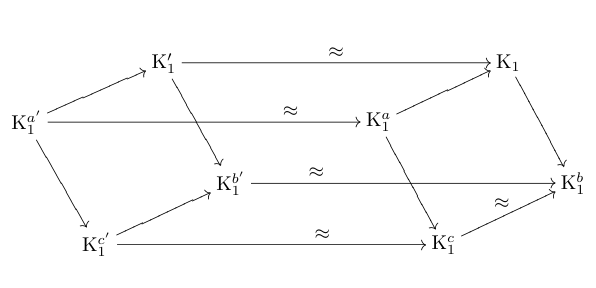
\includegraphics[width=.78\linewidth]{figures/sga4-3/08-gluing-resolutions-p217-resolution-cube.png}\end{center}
这里 $K'_1,K_1^{a'},K_1^{b'},K_1^{c'}$ 对\Term{functor}{函子} $L\otimes^{\mathbf L}Lg^*$ \Term{derived-adapted}{适配}；相应地，
\SourcePage{218}
\begin{center}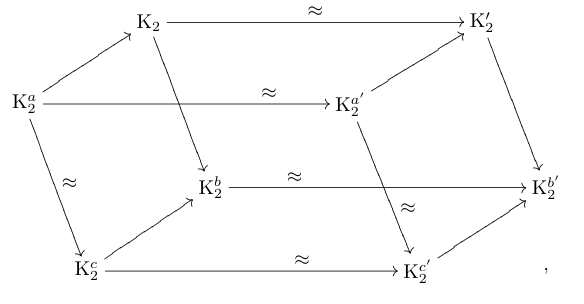
\includegraphics[width=.78\linewidth]{figures/sga4-3/08-gluing-resolutions-p218-resolution-cube.png}\end{center}
这里 $K'_2,K_2^{a'},K_2^{b'},K_2^{c'}$ 对\Term{functor}{函子} $Rf'_*$ \Term{derived-adapted}{适配}。用通常的\Term{base-change}{换基}\Term{morphism}{态射}，得到 $S$ 上\Term{complex}{复形}的交换棱柱图：
\begin{center}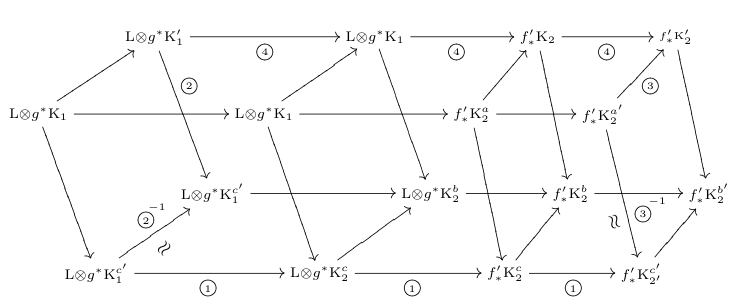
\includegraphics[width=\linewidth]{figures/sga4-3/08-gluing-resolutions-p218-prism.png}\end{center}
注意 (4.2.13.1) 中的\Term{arrow}{箭头}分别等同于下列复合\Term{arrow}{箭头}，便得结论：

$\varphi$ 对应于标号 \textcircled{1} 的\Term{arrow}{箭头}之复合；

$L\otimes^{\mathbf L}Lg^*(u')$ 对应于标号 \textcircled{2} 的\Term{arrow}{箭头}之复合，其中一条为某个\Term{quasi-isomorphism}{拟同构}的逆；

$Rf'_*(v')$ 对应于标号 \textcircled{3} 的\Term{arrow}{箭头}之复合，其中一条为某个\Term{quasi-isomorphism}{拟同构}的逆；

$c'_{u,v}$ 对应于标号 \textcircled{4} 的\Term{arrow}{箭头}之复合。
\SourcePage{219}
一般情形，令 $K'_1=f_*K,K'_2=f'^*L\otimes g'^*K$。此时有图
\begin{center}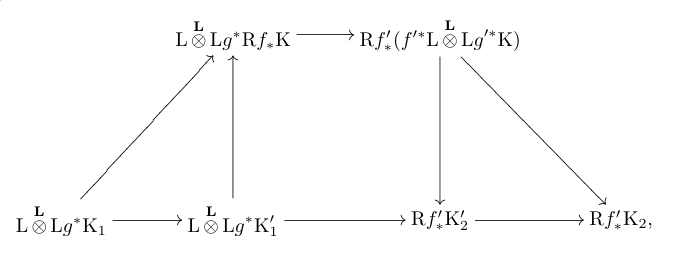
\includegraphics[width=.92\linewidth]{figures/sga4-3/08-gluing-resolutions-p219-general-diagram.png}\end{center}
其中各三角形交换，由上面的证明，内部矩形也交换。因此外\Term{boundary}{边界}交换，4.2.13 得证。
\end{proof}
\textbf{4.3. \Term{base-change-theorem}{换基定理}。}我们拟用\Term{derived-category}{导出范畴}的语言重新表述\Term{proper}{固有态射}的\Term{base-change}{换基}定理 XII 5.1 (iii)。
\begin{SGAresult}{定理}{4.3.1}
设有\Term{scheme}{概形}的\Term{cartesian}{笛卡尔}图
\[\begin{tikzcd}X'\arrow[r,"g'"]\arrow[d,"f'"']&X\arrow[d,"f"]\\S'\arrow[r,"g"]&S,\end{tikzcd}\]
其中 $f$ \Term{proper}{固有}。设 $\mathscr A,\mathscr A'$ 分别为 $S,S'$ 上的\Term{torsion}{挠}环\Term{sheaf}{层}，$L$ 为\Term{bounded-above}{上有界}的 $(\mathscr A',g^*\mathscr A)$-\Term{bimodule}{双模}\Term{complex}{复形}。假设 $f$ 的\Term{fiber}{纤维}\Term{dimension}{维数}\Term{bounded}{有界}。此时假设 4.2.12 (a) 成立，且从 $D^-(X,f^*\mathscr A)$ 到 $D^-(S',\mathscr A')$ 的\Term{functor}{函子}之间的\Term{base-change}{换基}\Term{arrow}{箭头} (4.2.12.3)
\[\varphi_K:L\otimes^{\mathbf L}Lg^*K\longrightarrow Rf'_*(f'^*L\otimes^{\mathbf L}Lg'^*K)\]
是\Term{isomorphism}{同构}。
\end{SGAresult}
\begin{proof}
所考虑的\Term{functor}{函子}三角化且为“way-out”\Term{functor}{函子} [RD I 7]，故为检验 $\varphi_K$ 为\Term{isomorphism}{同构}，只需检验各 $\varphi_{H^i(K)}$ 为\Term{isomorphism}{同构}。因此可假设 $K$ 是放在零次的一个（\Term{torsion}{挠}）$f^*\mathscr A$-模\Term{sheaf}{层}。

为检验 $\varphi_K$ 为\Term{isomorphism}{同构}，只需对 $\mathscr A'$-\Term{module-category}{模范畴}到 $\mathbf Z/n\mathbf Z$-\Term{module-category}{模范畴}的\Term{forgetful-functor}{遗忘函子}应用后检验，其中 $n\mathscr A=n\mathscr A'=0$。

这将我们归结为 $\mathscr A'=\mathbf Z/n\mathbf Z$ 且 $n\mathscr A=0$ 的情形。此时可用\Term{derived-category}{导出范畴}中\Term{isomorphism}{同构}的、\Term{set-component}{分量}在 $g^*\mathscr A$ 上\Term{flat}{平坦}且\Term{bounded-above}{上有界}的\Term{complex}{复形}代替 $L$。
\SourcePage{220}
所考虑\Term{functor}{函子}关于 $L$ 三角化且为 way-out \Term{functor}{函子}，故只须把 $L$ 换成其任一\Term{set-component}{分量}后验证 $\varphi_K$ 为\Term{isomorphism}{同构}。因此可假设 $L$ 是放在零次的一个\Term{flat}{平坦} $g^*\mathscr A$-模\Term{sheaf}{层}。需证\Term{arrow}{箭头}
\[\varphi^q:L\otimes g^*R^qf_*K\longrightarrow R^qf'_*(f'^*L\otimes g^*K)\]
为\Term{isomorphism}{同构}。设 $s$ 为 $S'$ 的\Term{geometric-point}{几何点}，$X_s$ 为 $X'$ 在 $s$ 处的\Term{fiber}{纤维}，$K_s$ 为 $K$ 在 $X_s$ 上的\Term{inverse-image}{逆像}。由 XII 5.1 (iii)，$\varphi^q$ 在 $s$ 处的\Term{fiber}{纤维}为\Term{arrow}{箭头}
\[\varphi_s^q:L_s\otimes H^q(X_s,K)\longrightarrow H^q(X_s,L_s\otimes K).\]
由 D. Lazard 的定理 [1]，\Term{flat}{平坦} $\mathscr A_s$-模 $L_s$ 为自由 $\mathscr A_s$-模 $L_{s,i}$ 的\Term{filtered-colimit}{滤过归纳极限}；\Term{functor}{函子} $H^q(X_s,*)$ 与\Term{filtered-colimit}{滤过归纳极限}可交换。因此 $\varphi^q$ 为\Term{arrow}{箭头}
\[\varphi_i^q:L_{s,i}\otimes H^q(X_s,K)\longrightarrow H^q(X_s,L_{s,i}\otimes K)\]
的\Term{inductive-limit}{归纳极限}。后者显然均为\Term{isomorphism}{同构}，故 $\varphi_s^q$ 也为\Term{isomorphism}{同构}，而 $\varphi$ 是\Term{isomorphism}{同构}。
\end{proof}
\textbf{变式 4.3.2。}(i) 当 $L$ 为\Term{bounded}{有界}\Term{complex}{复形}且各\Term{set-component}{分量}在 $g^*\mathscr A$ 上有\Term{finite}{有限}\Term{tor-dimension}{Tor 维数}时，4.2.12 (c) 的假设成立，可在整个\Term{derived-category}{导出范畴}中工作。

(ii) 若 $L$ \Term{bounded-below}{下有界}，各\Term{set-component}{分量}在 $g^*\mathscr A$ 上有\Term{finite}{有限}\Term{tor-dimension}{Tor 维数}，则即使 $\mathscr A,\mathscr A'$ 不是\Term{torsion}{挠}的，4.2.12 (b) 的假设仍成立；若各 $H^i(K)$ 为\Term{torsion}{挠}\Term{sheaf}{层}，\Term{base-change}{换基}\Term{arrow}{箭头} $\varphi_K$（$K\in D^+(X,f^*\mathscr A)$）是\Term{isomorphism}{同构}。
\SGAsection{5}{具有固有支撑的直接像函子}
\textbf{5.1. 基本构造。}拟按照 3.1 所述方案，对\Term{compactifiable-morphism}{可紧化态射} $f$（3.2）定义\Term{functor}{函子} $Rf_!$。附录将说明如何处理任意\Term{separated}{分离}\Term{finite-type}{有限型态射}。

\textbf{5.1.1.} 设 $X$ 为\Term{topos}{拓扑斯}，$U$ 为 $X$ 的开\Term{subobject}{子对象}（IV 8.3），$j$ 为 $U$ 到 $X$ 的\Term{inclusion-morphism}{包含态射}。IV 5.2 已定义一个从 $U$ 上\Term{set}{集合}\Term{sheaf}{层}\Term{category}{范畴}到 $X$ 上\Term{set}{集合}\Term{sheaf}{层}\Term{category}{范畴}的“\Term{extension-by-empty-set}{以空集延拓}”\Term{functor}{函子} $j_!$。它是\Term{restriction}{限制}\Term{functor}{函子} $j^*$ 的\Term{left-adjoint}{左伴随}。

仍以 $j_!$ 表示从 $U$ 上的\Term{pointed-set}{带基点集合}\Term{sheaf}{层}（相应地群\Term{sheaf}{层}，或 $j^*\mathscr A$-模\Term{sheaf}{层}，其中 $\mathscr A$ 是 $X$ 上的环\Term{sheaf}{层}）\Term{category}{范畴}到 $X$ 上对应\Term{category}{范畴}的、与\Term{restriction}{限制}\Term{functor}{函子} $j^*$ \Term{left-adjoint}{左伴随}的\Term{functor}{函子}（IV \SGAsourcegap{5.1.1 的 IV 后交叉引用编号缺失；原本及 SLMath 补源均为空白}）。这三个 $j_!$ 与从\Term{module-category}{模范畴}到群\Term{category}{范畴}、从群\Term{category}{范畴}到\Term{pointed-set}{带基点集合}\Term{category}{范畴}的\Term{forgetful-functor}{遗忘函子}相容\footnote{但与到\Term{set}{集合}\Term{category}{范畴}的\Term{forgetful-functor}{遗忘函子}不相容！}。
\SourcePage{221}
若 $i:F\to X$ 是 $U$ 的补闭\Term{subobject}{子对象}的包含，则 $j^*j_!$ （\Term{canonical-isomorphism}{典范同构}于）\Term{identity-functor}{恒等函子}，$i^*j_!$ 是值为\Term{initial-object}{始对象}（或\Term{final-object}{终对象}，这里二者相同）的\Term{constant-functor}{常值函子}。这也刻画 $j_!$。由此得出，所考虑的三个\Term{functor}{函子} $j_!$ \Term{exact}{正合}，且\Term{embedding}{嵌入}对应的\Term{functor}{函子} $j_*$。它们称为\Term{extension-zero}{零延拓}\Term{functor}{函子}。公式 $(j_1j_2)^*=j_2^*j_1^*$ \Term{transpose}{转置}为传递\Term{isomorphism}{同构}
\[(j_1j_2)_!=j_{1!}j_{2!}.\]
\Term{functor}{函子} $j_!$ 与\Term{base-change}{换基}相容：
\begin{SGAresult}{引理}{5.1.2}
设 $f:X\to Y$ 为\Term{topos}{拓扑斯}\Term{morphism}{态射}，$V$ 为 $Y$ 的开\Term{subobject}{子对象}，$U$ 为它在 $X$ 中的\Term{inverse-image}{逆像}：
\[\begin{tikzcd}U\arrow[r,"f'"]\arrow[d,"j'"']&V\arrow[d,"j"]\\X\arrow[r,"f"]&Y.\end{tikzcd}\]
则存在惟一\Term{base-change}{换基}\Term{isomorphism}{同构} $f^*j_!\xrightarrow{\sim}j'_!f'^*$，使下图交换：
\[\begin{tikzcd}f^*j_!\arrow[r,"\sim"]\arrow[d,hook]&j'_!f'^*\arrow[d,hook]\\f^*j_*\arrow[r,"\alpha"]&j'_*f'^*,\end{tikzcd}\tag{5.1.2.1}\]
其中 $\alpha$ 是\Term{base-change}{换基}\Term{arrow}{箭头}。
\end{SGAresult}
\begin{proof}
\Term{base-change}{换基}\Term{arrow}{箭头} $\varphi:j^*f_*\to f'_*j'^*$ 显然为\Term{isomorphism}{同构}。它\Term{transpose}{转置}为\Term{base-change}{换基}\Term{isomorphism}{同构} $\varphi':j'_!f'^*\xrightarrow{\sim}f^*j_!$。为检验 (5.1.2.1) 交换，只需检验其在 $U$ 上的\Term{restriction}{限制}交换，而这是平凡的。
\end{proof}
\textbf{5.1.3.} 在 5.1.1 的假设下，设 $X$ 由环\Term{sheaf}{层} $\mathscr A$ \Term{ringed}{赋环}。模上的\Term{functor}{函子} $j_!$ \Term{exact}{正合}，故可直接\Term{descent}{下降}到\Term{derived-category}{导出范畴}，定义仍记作 $j_!$ 的\Term{functor}{函子} $D(U,j^*\mathscr A)\to D(X,\mathscr A)$。仍有传递\Term{isomorphism}{同构}
\[(j_1j_2)=j_{1!}j_{2!}.\tag{5.1.3.1}\]
\SourcePage{222}
在\Term{derived-category}{导出范畴}层面还有\Term{adjunction}{伴随}公式
\[\operatorname{Hom}_{D(X)}(j_!K,L)\xrightarrow{\sim}\operatorname{Hom}_{D(U)}(K,j^*L).\tag{5.1.3.2}\]
\textbf{5.1.4.} 设 $f:X\to Y$ 是\Term{proper}{固有态射}，$\mathscr A$ 为 $Y$ 上的\Term{torsion}{挠}环\Term{sheaf}{层}，以 $\mathscr A$ 的\Term{inverse-image}{逆像}环\Term{sheaf}{层}\Term{ringed}{赋环} $X$。假设 $f$ 的\Term{fiber}{纤维}\Term{dimension}{维数}以整数 $n$ 为上界（若 $Y$ \Term{quasi-compact}{拟紧}，情况总是如此）。已知对 $X$ 上任意 $f^*\mathscr A$-模\Term{sheaf}{层} $F$，$q>2n$ 时 $R^qf_*F=0$（XII 5.3 bis；此引用据 SLMath 补源 PDF 第 345 页补全）。因此\Term{functor}{函子} $f_*$ 有\Term{derived-functor}{导出函子}（1.2.10）
\[Rf_*:D(X,f^*\mathscr A)\longrightarrow D(Y,\mathscr A).\]
若 $f$ 是两个\Term{proper}{固有态射}的复合 $gh$，则有传递公式 $Rf_*=Rg_*Rh_*$；如常可用\Term{cofibered-category}{余纤维范畴}表达它（评注 5.1.3）。

\textbf{5.1.5.} 设有\Term{scheme}{概形}的\Term{commutative-diagram}{交换图}
\[\begin{tikzcd}U\arrow[r,hook,"j_1"]\arrow[d,"g"']&X\arrow[d,"f"]\\V\arrow[r,hook,"j_2"]&Y,\end{tikzcd}\tag{5.1.5.1}\]
其中 $j_1,j_2$ 为\Term{open-immersion}{开浸入}，$f,g$ 为\Term{fiber}{纤维}\Term{dimension}{维数}以整数 $n$ 为上界的\Term{proper}{固有态射}。设 $\mathscr A$ 是 $Y$ 上的\Term{torsion}{挠}环\Term{sheaf}{层}，以其\Term{inverse-image}{逆像}\Term{ringed}{赋环} $U,V,X$。由 (5.1.3.2)，对于 $K\in D(U)$，定义\Term{arrow}{箭头}
\[d:j_{2!}Rg_*K\longrightarrow Rf_*j_{1!}K\tag{5.1.5.2}\]
\Term{equivalence}{等价}于定义\Term{arrow}{箭头} $d':Rg_*K\to j_2^*Rf_*j_{1!}K$。

\Term{fiber-product}{纤维积} $X'=V\times_Y X$ 纳入\Term{commutative-diagram}{交换图}
\[\begin{tikzcd}U\arrow[r,hook,"k"]\arrow[d,"g"']&X'\arrow[r,hook,"j'_2"]\arrow[d,"f'"]&X\arrow[d,"f"]\\V\arrow[r,equal]&V\arrow[r,hook,"j_2"]&Y,\end{tikzcd}\tag{5.1.5.3}\]
且显然 $j_2^*Rf_*j_{1!}K\simeq Rf'_*(j_2'^*j_{1!}K)\simeq Rf'_*k_!K$。
\SourcePage{223}
\Term{arrow}{箭头} $k$ 是\Term{proper}{固有}\Term{open-immersion}{开浸入}，所以 $k_!=k_*$，从而有\Term{isomorphism}{同构} $Rf'_*k_!K\simeq Rf'_*k_*K\simeq Rg_*K$。这给出所求\Term{isomorphism}{同构} $d'$ 及\Term{morphism}{态射} $d$。还可看出 $d$ 在 $V$ 上的\Term{restriction}{限制}是\Term{isomorphism}{同构}。
\begin{SGAresult}{引理}{5.1.6}
\Term{morphism}{态射} (5.1.5.2) 是\Term{isomorphism}{同构}。
\end{SGAresult}
\begin{proof}
只需验证 $d$ 在 $Y-V=F$ 上的\Term{restriction}{限制}为\Term{isomorphism}{同构}。令 $X''=X\times_Y F$，对\Term{cartesian}{笛卡尔}方块
\[\begin{tikzcd}X''\arrow[r,"i'"]\arrow[d,"f''"']&X\arrow[d,"f'"]\\F\arrow[r,"i"]&Y\end{tikzcd}\]
应用\Term{proper}{固有态射}\Term{base-change}{换基}定理（4.3.1），取 $\mathscr A'=i^*\mathscr A,L=\mathscr A'[0]$。得到
\[i^*Rf_*j_{1!}K\simeq Rf''_*i'^*j_{1!}K\simeq Rf''_*0\simeq0.\]
故 (5.1.5.2) 的两端在 $U$ 之外均为零，且 $d$ 是\Term{isomorphism}{同构}。
\end{proof}
\textbf{5.1.7.} 设 $S$ 是由\Term{torsion}{挠}环\Term{sheaf}{层} $\mathscr A$ \Term{ringed}{赋环}的\Term{scheme}{概形}。对每个 $S$-\Term{scheme}{概形} $\phi:X\to S$，令 $\mathscr A_X=\phi^*\mathscr A$。在\Term{quasi-compact}{拟紧}\Term{quasi-separated}{拟分离} $S$-\Term{scheme}{概形}及 $S$-\Term{compactifiable-morphism}{可紧化态射}所成的\Term{category}{范畴} $(S)$ 中工作（3.2）。由 3.2.3，此\Term{category}{范畴}以及\Term{open-immersion}{开浸入}\Term{subcategory}{子范畴} $(S,i)$、\Term{proper}{固有态射}\Term{subcategory}{子范畴} $(S,p)$ 满足 3.2.4 的假设。

拟对下列资料应用理论 3.3.2（采用 3.3.1 的记号）：

$\alpha)$ 对 $\phi:X\to S$，$F(X)=D(X,\mathscr A_X)$；

(i) 对\Term{proper}{固有}的 $p:X\to Y$，取 $p_*$ 为\Term{functor}{函子} $Rp_*$；

(ii) 采用通常传递\Term{isomorphism}{同构} $R(pq)_*=Rp_*Rq_*$；

(i$'$) 对\Term{open-immersion}{开浸入} $i:X\to Y$，取 $i_*$ 为\Term{functor}{函子} $i_!$；

(ii$'$) 采用传递\Term{isomorphism}{同构} (5.1.3.1)；

(iii) 对每个\Term{commutative-diagram}{交换图} (5.1.5.1)，取 $d$ 为\Term{isomorphism}{同构} (5.1.5.2)。

检验 3.3.2 的条件 (a)、(b)、(c)、(a$'$)、(b$'$)、(c$'$)，便得到下列定理的 (a) 部分。
\begin{SGAresult}{定理}{5.1.8}
(a) 在 5.1.7 定义的\Term{category}{范畴} $(S)$ 中，可以用一种且本质上惟一的方式，对每个\Term{arrow}{箭头} $f:X\to Y$ 定义\Term{functor}{函子}
\[Rf_!:D(X,\mathscr A_X)\longrightarrow D(Y,\mathscr A_Y),\]
\SourcePage{224}
并对每个\Term{composition-morphism}{复合态射} $f=gh:X\xrightarrow{h}Y\xrightarrow{g}Z$ 定义 $Rf_!$ 与 $Rg_!Rh_!$ 之间的传递\Term{isomorphism}{同构} $c_{f,g}$，使得：

(i) 各 $c_{f,g}$ 满足“\Term{cocycle-condition}{上闭链条件}”
\[(c_{f,g}*Rh_!)\circ c_{fg,h}=(Rf_!*c_{g,h})\circ c_{f,gh}.\]
(ii) \Term{restriction}{限制}到\Term{proper}{固有态射}（相应地\Term{open-immersion}{开浸入}）时，得到变性理论 5.1.4（相应地 5.1.3）。

(iii) 对每个图 (5.1.5.1)，\Term{isomorphism}{同构} $d$（5.1.5.2）是\Term{composition-isomorphism}{复合同构} $c_{f,j'}\circ c_{j,f'}^{-1}$。

(b) 各\Term{functor}{函子} $Rf_!$ 都是“way out”\Term{functor}{函子} [RD I 7]，且为\Term{triangulated-functor}{三角函子}。
\end{SGAresult}
\begin{proof}
任意 $Rf_!$ 均为\Term{functor}{函子} $Rg_*$ 与 $j_!$ 的复合，其中 $g$ \Term{proper}{固有}、靶\Term{quasi-compact}{拟紧}，故\Term{fiber}{纤维}\Term{dimension}{维数}\Term{bounded}{有界}，$j$ 为\Term{open-immersion}{开浸入}。这些\Term{functor}{函子}都是 way out \Term{triangulated-functor}{三角函子}，故 $Rf_!$ 也是。
\end{proof}
\textbf{5.1.8.1.} 5.1.8 (a) 的传递\Term{isomorphism}{同构}，常通过由此\Term{derive}{导出}的“\Term{composite-functor}{复合函子}”\Term{spectral-sequence}{谱序列}来使用；对 $K\in\operatorname{Ob}D(X,\mathscr A_X)$ 有
\[E_2^{pq}=R^pg_!R^qh_!(K)\Longrightarrow R^{p+q}f_!(K).\tag{5.1.8.2}\]
要得到它，只需注意，由 5.1.8 (b) 和 [VERDIER 2]，对每个 $L\in\operatorname{Ob}D(Y,\mathscr A_Y)$ 有\Term{spectral-sequence}{谱序列}
\[E_2^{pq}=R^pg_!(H^q(L))\Longrightarrow R^{p+q}g_!(L),\tag{5.1.8.3}\]
而 (5.1.8.2) 是取 $L=Rh_!K$ 的特例。
\begin{SGAresult}{定义}{5.1.9}
(i) 5.1.8 构造的\Term{functor}{函子}称为“全\Term{proper-support}{固有支撑}\Term{direct-image}{直接像}\Term{functor}{函子}”。不致混淆时，省去形容词“全”。

(ii) \Term{composite-functor}{复合函子} $H^q\circ Rf_!$ 称为第 $q$ 个\Term{proper-support}{固有支撑}\Term{direct-image}{直接像}\Term{functor}{函子}，记为 $R^qf_!$。

(iii) 若 $X$ 是可\Term{immersion}{浸入} $k$ 上\Term{proper}{固有}\Term{scheme}{概形}的、\Term{separably-closed-field}{可分闭域} $k$ 上的\Term{scheme}{概形}，则将 $\operatorname{Spec}(k)$ 上的模\Term{sheaf}{层}与通常的模等同，\Term{functor}{函子} $R^qf_!$ 记为 $H_c^q(X,\ )$、$H_!^q(X,\ )$，不致混淆时也简记 $H_c^q(\ )$。此时称之为“第 $q$ 个\Term{proper-support}{固有支撑}\Term{hypercohomology}{超上同调}群”；若用于集中在零次的\Term{complex}{复形}，则称为“第 $q$ 个\Term{proper-support}{固有支撑}\Term{cohomology-group}{上同调群}”。
\end{SGAresult}
\textbf{5.1.9.1.} 记号 $Rf_!$ 有滥用之处，因为它并不是将在 6.1.2 定义的\Term{functor}{函子} $f_!$ 的右\Term{derived-functor}{导出函子}。有些人更喜欢用 $R_!f$。
\SourcePage{225}
\textbf{5.1.10.} 5.1.8 的证明所用材料，是\Term{proper}{固有}\Term{base-change}{换基}定理，以及当 $j$ 是\Term{proper}{固有}\Term{open-immersion}{开浸入}时 $j_*=j_!$。由此可表述 5.1.8 的各种变式；赋予它们精确意义并加以验证的工作留给读者。
\begin{SGAresult}{变式}{5.1.11}
在\Term{category}{范畴} $(S)$ 中，可以用一种且本质上惟一的方式，对每个\Term{arrow}{箭头} $f:X\to Y$ 定义从 $X$ 上\Term{pointed-set}{带基点集合}\Term{sheaf}{层}\Term{category}{范畴}到 $Y$ 上\Term{pointed-set}{带基点集合}\Term{sheaf}{层}\Term{category}{范畴}的\Term{functor}{函子} $f_!$，并对任意\Term{composition-morphism}{复合态射} $f=gh$ 定义传递\Term{isomorphism}{同构}，满足与 5.1.4 中 (i)、(ii)、(iii) 类似的条件。
\end{SGAresult}
此\Term{functor}{函子}的直接描述见 6.1.2。
\begin{SGAresult}{变式}{5.1.12}
对任意\Term{compactifiable-morphism}{可紧化态射} $f:X\to Y$，可定义从 $X$ 上 Ind-\Term{finite-group}{有限群}\Term{sheaf}{层}\Term{category}{范畴}到 $Y$ 上\Term{pointed-set}{带基点集合}\Term{sheaf}{层}\Term{category}{范畴}的\Term{functor}{函子} $R^1f_!$，并且对于 $f$ 的每个\Term{compactification}{紧化} $f=\bar f j$，有\Term{isomorphism}{同构} $R^qf_!\simeq R^1\bar f_*\circ f_!$。
\end{SGAresult}
\begin{proof}
这里不要求任何传递公式；惟一的问题是证明 $R^1f_!$ 不依赖于所选 $f$ 的\Term{compactification}{紧化}。设 $p:(\bar f_1,i_1)\to(\bar f_2,i_2)$ 是一个\Term{compactification}{紧化}\Term{morphism}{态射}，即图
\[\begin{tikzcd}X\arrow[r,"i_1"]\arrow[dr,"i_2"']\arrow[dd,"f"']&\bar X_1\arrow[d,"p"]\\&\bar X_2\arrow[dl,"\bar f_2"]\\Y&\end{tikzcd}\tag{5.1.12.1}\]
其中 $\bar f_1=\bar f_2\circ p$，且 $p$ \Term{proper}{固有}。若 $G$ 是 $X$ 上的群\Term{sheaf}{层}，则有\Term{pointed-set}{带基点集合}的\Term{exact-sequence}{正合列}（$\alpha$ \Term{injectivity}{单射}）
\[0\longrightarrow R^1\bar f_{2*}(p_*i_{1!}G)\xrightarrow{\alpha}R^1\bar f_{1*}(i_{1!}G)\longrightarrow\bar f_{2*}R^1p_*(i_{1!}G),\]
及从 $i_{2!}G$ 到 $p_*i_{1!}G$ 的\Term{arrow}{箭头}，从而复合得到 $\beta:R^1\bar f_{2*}i_{2!}G\to R^1\bar f_{1*}i_{1!}G$。如 3.3.2.1 论证，问题归结为证明当 $G$ 为 Ind-\Term{finite}{有限}时，此\Term{arrow}{箭头}总为\Term{isomorphism}{同构}。

对 $p$ 及\Term{set}{集合}\Term{sheaf}{层} $i_{1!}G$ 应用\Term{proper}{固有}\Term{base-change}{换基}定理，得 $p_*i_{1!}G=i_{2!}G$，故有\Term{exact-sequence}{正合列}
\[0\longrightarrow R^1\bar f_{2*}(i_{2!}G)\xrightarrow{\beta}R^1\bar f_{1*}(i_{1!}G)\longrightarrow\bar f_{2*}R^1p_*i_{1!}G.\]
\SourcePage{226}
\Term{arrow}{箭头} $\beta$ 为\Term{injectivity}{单射}（因为 $\alpha$ 为\Term{injectivity}{单射}）。再对 $p$ 及假定为 Ind-\Term{finite}{有限}的群\Term{sheaf}{层} $G$ 应用\Term{proper}{固有}\Term{base-change}{换基}定理，得到 $R^qp_*i_{1!}G=0$。因此 $\beta$ 为\Term{epimorphism}{满态射}，完成 5.1.12 的证明。
\end{proof}
\begin{SGAresult}{定义}{5.1.13}
对任意\Term{site}{景} $X$，以 $D_{\mathrm{tors}}(X)$ 表示 $X$ 上阿贝尔\Term{sheaf}{层}\Term{category}{范畴}的\Term{derived-category}{导出范畴}中，由\Term{cohomology}{上同调}\Term{sheaf}{层}均为\Term{torsion}{挠}的\Term{complex}{复形}构成的\Term{full-subcategory}{满子范畴}。
\end{SGAresult}
\begin{SGAresult}{变式}{5.1.14}
在\Term{category}{范畴} $(S)$ 中，可用一种且本质上惟一的方式，对每个\Term{arrow}{箭头} $f:X\to Y$ 定义三角且“way out” [RD I 7] 的\Term{functor}{函子}
\[Rf_!:D^+_{\mathrm{tors}}(X)\longrightarrow D^+_{\mathrm{tors}}(Y),\]
并对任意\Term{composition-morphism}{复合态射} $f=gh$ 定义传递\Term{isomorphism}{同构}，满足与 5.1.4 中 (i)、(ii)、(iii) 类似的条件。
\end{SGAresult}
\begin{SGAresult}{变式}{5.1.5}
考虑由\Term{torsion}{挠}环\Term{sheaf}{层}\Term{ringed}{赋环}的 $S$-\Term{scheme}{概形}\Term{category}{范畴}，其\Term{arrow}{箭头}是诱导（0.8）一个 $S$-\Term{compactifiable-morphism}{可紧化}\Term{scheme}{概形}\Term{morphism}{态射}的\Term{ringed}{赋环}\Term{scheme}{概形}\Term{morphism}{态射}。对每个\Term{arrow}{箭头} $f:(X,\mathscr A)\to(Y,\mathscr B)$，令 $Rf_!$ 为从 $\mathscr A$-\Term{module-category}{模范畴}到 $f^*\mathscr B$-\Term{module-category}{模范畴}的\Term{forgetful-functor}{遗忘函子}与 $Rf_!$ 的复合。这些\Term{functor}{函子}具有通常 $Rf_!$ 的变性性质。
\end{SGAresult}
但应注意，只有当 $\mathscr A$ 在 $f^*\mathscr B$ 上\Term{finite}{有限}时，这里的记号 $Rf_!$ 才合理；取 $X=Y=\operatorname{Spec}(k)$，$k$ \Term{algebraically-closed}{代数闭}，即可看出此点。

\textbf{5.1.16.} 设 $f:X\to S$ 为\Term{compactifiable-morphism}{可紧化态射}，$j:U\to X$ 为 $X$ 的开\Term{subobject}{子对象}，$i:F\to X$ 为其补闭\Term{subobject}{子对象}，$\mathscr A_S$ 为 $S$ 上的\Term{torsion}{挠}环\Term{sheaf}{层}，$\mathscr A_X$ 为其在 $X$ 上的\Term{inverse-image}{逆像}，$K\in\operatorname{Ob}D(X,\mathscr A_X)$。

\Term{complex}{复形}的\Term{exact-sequence}{正合列}
\[0\longrightarrow j_!j^*K\longrightarrow K\longrightarrow i_!i^*K\longrightarrow0\]
在 $D(X,\mathscr A_X)$ 中产生一个\Term{distinguished-triangle}{区别三角} [VERDIER C.D. I 2.4]。它在 $Rf_!$ 下的像是\Term{distinguished-triangle}{区别三角}（5.1.8 (b)）
\[R(fj)_!j^*K\longrightarrow Rf_!K\longrightarrow R(fi)_!i^*K\longrightarrow R(fj)_!j^*K[1]\cdots,\tag{5.1.16.1}\]
从而定义\Term{cohomology}{上同调}长\Term{exact-sequence}{正合列}
\[\cdots\longrightarrow R^q(fj)_!j^*K\longrightarrow R^qf_!K\longrightarrow R^q(fi)_!i^*K\xrightarrow{j}R^{q+1}(fj)_!j^*K\longrightarrow\cdots.\tag{5.1.16.2}\]
\SourcePage{227}
特别地，若 $S$ 为\Term{separably-closed-field}{可分闭域}的谱，且 $K$ 是放在零次的\Term{sheaf}{层} $G$，则 (5.1.16.2) 写成
\[\cdots H_c^q(U,G)\longrightarrow H_c^q(X,G)\longrightarrow H_c^q(F,G)\xrightarrow{j}H_c^{q+1}(U,G)\cdots.\tag{5.1.16.3}\]
\textbf{5.1.17.} 设有 $S$-\Term{compactifiable-morphism}{可紧化}\Term{scheme}{概形}的图
\[\begin{tikzcd}X\arrow[rr,"u"]\arrow[dr,"f"']&&Y\arrow[dl,"g"]\\&S&,\end{tikzcd}\]
且 $u$ \Term{proper}{固有}。以 $S$ 上\Term{torsion}{挠}环\Term{sheaf}{层} $\mathscr A_S$ 的\Term{inverse-image}{逆像}\Term{ringed}{赋环} $X,Y$。对于 $K\in D(Y,\mathscr A_Y)$，显然的\Term{adjoint}{伴随箭头} $K\to Ru_*u^*K$ 在施加 $Rg_!$ 后定义\Term{arrow}{箭头}
\[u^*:Rg_!K\longrightarrow Rg_!Ru_*u^*K=Rg_!Ru_!u^*K\simeq Rf_!u^*K\tag{5.1.17.1}\]
（\Term{proper-support}{固有支撑}\Term{cohomology}{上同调}对于\Term{proper}{固有态射}的\Term{contravariant}{反变}性）。若 $S$ 为\Term{algebraically-closed-field}{代数闭域}的谱，$K$ 是放在零次的\Term{sheaf}{层} $G$，则此\Term{arrow}{箭头}写成
\[u^*:H_c^q(Y,G)\longrightarrow H_c^q(X,G).\tag{5.1.17.2}\]

\textbf{5.2. \Term{base-change-theorem}{换基定理}。}
\textbf{5.2.1.} 设 $f:X\to Y$ 为\Term{topos}{拓扑斯}\Term{morphism}{态射}，$V$ 为 $Y$ 的开\Term{subobject}{子对象}，$U=f^{-1}(V)$ 为其在 $X$ 中的\Term{inverse-image}{逆像}，$\mathscr A$ 为 $Y$ 上环\Term{sheaf}{层}，$\mathscr A'$ 为 $X$ 上环\Term{sheaf}{层}，$L$ 为\Term{bounded-above}{上有界}的 $(\mathscr A',f^*\mathscr A)$-\Term{bimodule}{双模}\Term{complex}{复形}：
\[\begin{tikzcd}U\arrow[r,"f'"]\arrow[d,hook,"j'"']&V\arrow[d,hook,"j"]\\X\arrow[r,"f"]&Y.\end{tikzcd}\tag{5.2.1.1}\]
有从 $D(V,\mathscr A)$ 到 $D(X,f^*\mathscr A)$ 的\Term{functor}{函子}间的\Term{base-change}{换基}\Term{isomorphism}{同构}（5.1.2.1）$f^*j_!\xrightarrow{\sim}j'_!f'^*$。又有从 $D^-(U,f'^*\mathscr A)$ 到 $D^-(X,\mathscr A')$ 的\Term{functor}{函子}间的显然\Term{isomorphism}{同构}
\[L\otimes^{\mathbf L}_{f^*\mathscr A}j'_!K\simeq j'_!(j'^*L\otimes^{\mathbf L}_{f^*\mathscr A}K).\]
为构造它，只需注意：若\Term{complex}{复形} $K$ 对 $j'^*L\otimes^{\mathbf L}$ \Term{derived-adapted}{适配}，则 $j'_!K$ 对 $L\otimes^{\mathbf L}$ \Term{derived-adapted}{适配}，
\SourcePage{228}
且在\Term{complex}{复形}层面有上述类型的\Term{isomorphism}{同构}。复合这两个\Term{isomorphism}{同构}，得到从 $D^-(V,\mathscr A)$ 到 $D^-(X,\mathscr A')$ 的\Term{functor}{函子}间的\Term{base-change}{换基}\Term{isomorphism}{同构}
\[L\otimes^{\mathbf L}_{f^*\mathscr A}f^*j_!K\xrightarrow{\sim}j'_!(j'^*L\otimes^{\mathbf L}_{f'^*\mathscr A}f'^*K).\tag{5.2.1.2}\]
若 $L$ \Term{bounded}{有界}且各\Term{set-component}{分量}在 $f^*\mathscr A$ 上有\Term{finite}{有限}\Term{tor-dimension}{Tor 维数}，则此\Term{isomorphism}{同构}对 $K\in\operatorname{Ob}D(V,\mathscr A)$ 仍有定义。

\textbf{5.2.2.} 设 $f:X\to S,g:S'\to S$ 为\Term{scheme}{概形}\Term{morphism}{态射}，并假设 $f$ 为\Term{open-immersion}{开浸入} $j$ 与\Term{proper}{固有态射} $p$ 的复合，且 $p$ 的\Term{fiber}{纤维}\Term{dimension}{维数}以某个整数 $n$ 为上界（$S$ \Term{quasi-compact}{拟紧}时自动成立）。这些\Term{morphism}{态射}纳入各方块\Term{cartesian}{笛卡尔}的图
\[\begin{tikzcd}X'\arrow[rr,"g'"]\arrow[drr,hook,"j'"']\arrow[dd,"f'"']&&X\arrow[drr,hook,"j"]\arrow[dd,"f"]&&\\&&\bar X'\arrow[rr,"\bar g"]\arrow[dll,"p'"']&&\bar X\arrow[dll,"p"]\\S'\arrow[rr,"g"']&&S&&\end{tikzcd}\]
设 $\mathscr A$ 为 $S$ 上\Term{torsion}{挠}环\Term{sheaf}{层}，$\mathscr A'$ 为 $S'$ 上\Term{torsion}{挠}环\Term{sheaf}{层}，$L$ 为\Term{bounded-above}{上有界}的 $(\mathscr A',g^*\mathscr A)$-\Term{bimodule}{双模}\Term{complex}{复形}。以 $\mathscr A$（相应地 $\mathscr A'$）在 $X,\bar X$（相应地 $X',\bar X'$）上的\Term{inverse-image}{逆像} $\mathscr A_X,\mathscr A_{\bar X}$（相应地 $\mathscr A'_{X'},\mathscr A'_{\bar X'}$）\Term{ringed}{赋环}这些\Term{scheme}{概形}。于是有 (5.2.1.2) 的\Term{base-change}{换基}\Term{isomorphism}{同构}，连接从 $D^-(X,\mathscr A_X)$ 到 $D^-(\bar X',\mathscr A'_{\bar X'})$ 的\Term{functor}{函子}
\[p'^*L\otimes^{\mathbf L}\bar g^*j_!K\quad\text{与}\quad j'_!(f'^*L\otimes^{\mathbf L}g'^*K),\]
以及 (4.3.1) 的\Term{base-change}{换基}\Term{isomorphism}{同构}，连接从 $D^-(\bar X,\mathscr A_{\bar X})$ 到 $D^-(S',\mathscr A')$ 的\Term{functor}{函子}
\[L\otimes^{\mathbf L}g^*Rp_*K\quad\text{与}\quad Rp'_*(p'^*L\otimes^{\mathbf L}\bar g^*K).\]
复合即得从 $D^-(X,\mathscr A_X)$ 到 $D^-(S',\mathscr A')$ 的\Term{functor}{函子}间的\Term{base-change}{换基}\Term{isomorphism}{同构}
\[L\otimes^{\mathbf L}g^*Rp_*j_!K\xrightarrow{\sim}Rp'_*j'_!(f'^*L\otimes^{\mathbf L}g'^*K).\tag{5.2.2.1}\]
当 $L$ \Term{bounded}{有界}且各\Term{set-component}{分量}有\Term{finite}{有限}\Term{tor-dimension}{Tor 维数}时，以上论证及 4.3.2 (i) 允许对 $K\in\operatorname{Ob}D(X,\mathscr A_X)$ 定义此\Term{base-change}{换基}\Term{isomorphism}{同构}。

为了引用 5.1.8，假设 $S$ \Term{quasi-compact}{拟紧}\Term{quasi-separated}{拟分离}。此时\Term{functor}{函子} $Rp_*j_!=Rf_!,Rp'_*j'_!=Rf'_!$ 只依赖于 $f,f'$，于是下述引理有意义。
\SourcePage{229}
\begin{SGAresult}{引理}{5.2.3}
\Term{base-change}{换基}\Term{isomorphism}{同构} (5.2.2.1) 不依赖于所选 $X$ 的\Term{compactification}{紧化} $f=pj$。
\end{SGAresult}
\begin{proof}
设 $q:\bar X_1\to\bar X_2$ 是\Term{compactification}{紧化}\Term{morphism}{态射}：
\[\begin{tikzcd}X\arrow[r,"j_1"]\arrow[dr,"j_2"]\arrow[dd,"f"']&\bar X_1\arrow[d,"q"]\arrow[ddl,"p_1",bend left=20]\\&\bar X_2\arrow[dl,"p_2"]\\S&.\end{tikzcd}\tag{5.2.3.1}\]
关于 $\bar X_1$ 的\Term{base-change}{换基}\Term{isomorphism}{同构} $c_1$，可由关于 $j_1,p_1$ 的\Term{isomorphism}{同构}“复合”得到，也可由关于 $j_1,q,p_2$ 的\Term{isomorphism}{同构}复合得到。关于 $\bar X_2$ 的\Term{isomorphism}{同构} $c_2$ 由关于 $j_2,p_2$ 的\Term{isomorphism}{同构}复合得到。为检验 $c_1=c_2$，只须检验关于 $j_2$ 的\Term{isomorphism}{同构} $c'_1$ 等于由关于 $j_1,q$ 的\Term{isomorphism}{同构}所成的复合 $c'_2$。以撇号表示 (5.2.3.1) 的\Term{arrow}{箭头}沿 $g$ \Term{base-change}{换基}后得到的\Term{arrow}{箭头}；则 $c'_1,c'_2$ 是\Term{isomorphism}{同构}
\[c'_1,c'_2:L\otimes^{\mathbf L}\bar g_2^*j_{2!}K\xrightarrow{\sim}j'_{2!}(j_2'^*L\otimes^{\mathbf L}g'^*K).\]
由 (5.1.3.2)，为检验 $c'_1=c'_2$，只需\Term{restriction}{限制}到 $X'_2$ 后检验，而这是平凡的。

因此，两个\Term{compactification}{紧化}间若有\Term{morphism}{态射}，则相应的\Term{base-change}{换基}\Term{isomorphism}{同构}相同；由 3.2.6 (ii) 即得结论。
\end{proof}
\begin{SGAresult}{引理}{5.2.4}
设 $f=uv:X\to Y\to S$ 为 $S$-\Term{compactifiable-morphism}{可紧化态射}的复合。关于 $u,v,f$ 的\Term{base-change}{换基}\Term{isomorphism}{同构} (5.2.2.1) 构成下列\Term{commutative-diagram}{交换图}（记号见下面 (5.2.4.1)）：
\begin{center}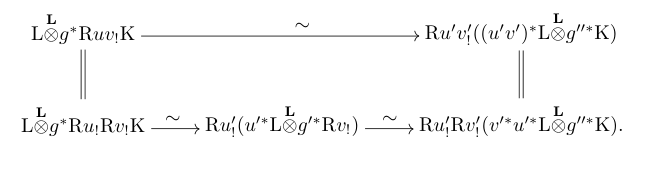
\includegraphics[width=\linewidth]{figures/sga4-3/08-gluing-resolutions-p229-base-composition.png}\end{center}
\end{SGAresult}
\begin{proof}
选取 $(u,v)$ 的一个\Term{compactification}{紧化}（3.2.5）：
\SourcePage{230}
\begin{center}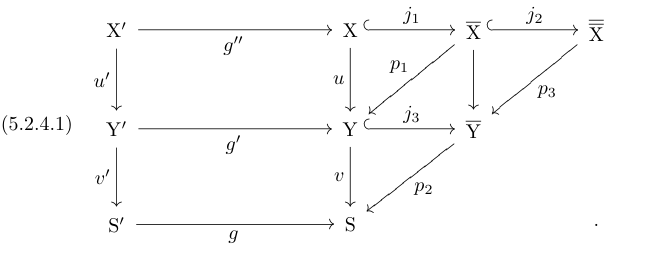
\includegraphics[width=.9\linewidth]{figures/sga4-3/08-gluing-resolutions-p230-compactification.png}\end{center}
引理 5.2.4 断言，关于 $f$ 的\Term{base-change}{换基}\Term{isomorphism}{同构} $c_1$ 是关于 $u,v$ 的\Term{isomorphism}{同构}的复合 $c_2$。$c_1$ 由关于 $j_1,j_2,p_3,p_2$ 的\Term{base-change}{换基}\Term{isomorphism}{同构}复合得到；$c_2$ 则由关于 $j_1,p_1,j_3,p_2$ 的\Term{isomorphism}{同构}复合得到。因此只须比较：关于 $p_3,j_2$ 的\Term{isomorphism}{同构}的复合 $c'_1$，以及关于 $j_3,p_1$ 的\Term{isomorphism}{同构}的复合 $c'_2$。

取\Term{cartesian}{笛卡尔}图
\begin{center}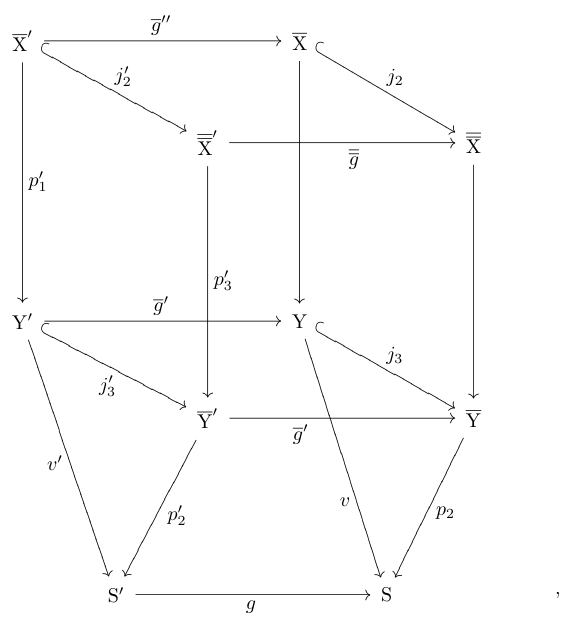
\includegraphics[width=.76\linewidth]{figures/sga4-3/08-gluing-resolutions-p230-cartesian-cube.png}\end{center}
令 $L'=p_2'^*$，并且
\SourcePage{231}
\[c'_1,c'_2:L'\otimes^{\mathbf L}\bar g'^*R(j_3p_1)_!K\xrightarrow{\sim}R(j'_3p'_1)_!((j'_3p'_1)^*L'\otimes g''^*K).\]
由 (5.1.3.2)，为检验 $c'_1=c'_2$，只须检验 $j_3'^*(c'_1)=j_3'^*(c'_2)$，这是平凡的。
\end{proof}
\begin{SGAresult}{引理}{5.2.5}
设有由\Term{torsion}{挠}环\Term{sheaf}{层}\Term{ringed}{赋环}的\Term{scheme}{概形}之间的\Term{morphism}{态射}
\[(S'',\mathscr A'')\xrightarrow{g_2}(S',\mathscr A')\xrightarrow{g_1}(S,\mathscr A),\]
以及\Term{compactifiable-morphism}{可紧化态射} $f:X\to S$，从而有图
\[\begin{tikzcd}X''\arrow[r,"g'_2"]\arrow[d,"f''"']&X'\arrow[r,"g'_1"]\arrow[d,"f'"]&X\arrow[d,"f"]\\S''\arrow[r,"g_2"]&S'\arrow[r,"g_1"]&S.\end{tikzcd}\]
以 $f^*\mathscr A,f'^*\mathscr A',f''^*\mathscr A''$ 分别\Term{ringed}{赋环} $X,X',X''$。则下图交换：
\[\begin{tikzcd}[column sep=small]L(g_1g_2)^*Rf_!\arrow[rr,"\sim"]\arrow[d,equal]&&Rf''_!L(g'_1g'_2)^*\arrow[d,equal]\\Lg_1^*Lg_2^*Rf_!\arrow[r,"\sim"]&Lg_1^*Rf'_!Lg_2^*\arrow[r,"\sim"]&Rf''_!Lg_1'^*Lg_2'^*.\end{tikzcd}\]
\end{SGAresult}
这个引理立即由关于 $j_!$ 与 $Rp_*$（$p$ \Term{proper}{固有}）的相应结果得出。细节留给读者。

上述陈述归纳为：
\begin{SGAresult}{定理}{5.2.6}
\Term{functor}{函子} $Rf_!$ 与\Term{base-change}{换基}可交换。
\end{SGAresult}
\textbf{变式 5.2.7。}(i) \Term{functor}{函子} $f_!$（对\Term{pointed-set}{带基点集合}\Term{sheaf}{层}，5.1.11）及 $R^1f_!$（对群\Term{sheaf}{层}，5.1.12）与\Term{base-change}{换基}可交换。

(ii) \Term{functor}{函子} $Rf_!$（5.1.14）与\Term{base-change}{换基}可交换。

(iii) 在 5.2.2 的假设下，若 $L$ \Term{bounded}{有界}且各\Term{set-component}{分量}有\Term{finite}{有限}\Term{tor-dimension}{Tor 维数}，则\Term{functor}{函子} $Rf_!:D(X)\to D(S)$ 与\Term{base-change}{换基}可交换。

定理 5.2.6 本质上\Term{equivalence}{等价}于下述 5.2.8、5.2.9 两个推论的合取。
\begin{SGAresult}{命题}{5.2.8}
设 $f:X\to S$ 为\Term{compactifiable-morphism}{可紧化态射}，$F$ 为 $X$ 上\Term{torsion}{挠}\Term{sheaf}{层}。对 $S$ 的每个\Term{geometric-point}{几何点} $s$，设 $X_s$ 为 $X$ 在 $s$ 处的\Term{geometric-fibre}{几何纤维}，$F_s$ 为诱导的\Term{sheaf}{层}。有\Term{canonical}{典范}等式
\[(R^qf_!F)_s=H_c^q(X_s,F_s).\]
\end{SGAresult}
\SourcePage{232}
\begin{SGAresult}{推论}{5.2.8.1}
若 $f$ 的\Term{fiber}{纤维}\Term{dimension}{维数} $\le d$，则\Term{functor}{函子} $Rf_!$ 的\Term{cohomological-dimension}{上同调维数} $\le2d$（1.2.9）：对每个\Term{torsion}{挠}\Term{sheaf}{层} $F$，当 $i>2d$ 时 $R^if_!F=0$。因此\Term{functor}{函子} $R^{2d}f_!$ 在\Term{torsion}{挠}\Term{sheaf}{层}\Term{category}{范畴}上\Term{right-exact}{右正合}。
\end{SGAresult}
\begin{proof}
通过\Term{base-change}{换基}（5.2.8），归结为 $S$ 是\Term{algebraically-closed-field}{代数闭域}的谱的情形。此时若 $\bar X$ 是 $S$ 上\Term{proper}{固有}的\Term{scheme}{概形}，包含 $X$ 作为 Zariski \Term{dense}{稠密}开子\Term{scheme}{概形} $j:X\to\bar X$，则 $\dim\bar X=\dim X\le D$。因此对 $X$ 上\Term{torsion}{挠}\Term{sheaf}{层} $F$ 和 $i>2d$，由 X 4.3、5.2 得
\[H_c^i(X,F)=H^i(\bar X,j_!F)=0.\]
\end{proof}
\begin{SGAresult}{命题}{5.2.9}
设 $f:X\to S$ 是\Term{compactifiable-morphism}{可紧化态射}，$\mathscr A$ 为 $S$ 上的\Term{torsion}{挠}环\Term{sheaf}{层}，$K$ 为\Term{bounded-above}{上有界}左 $f^*\mathscr A$-模\Term{complex}{复形}，$L$ 为\Term{bounded-above}{上有界}右 $\mathscr A$-模\Term{complex}{复形}。有\Term{canonical}{典范}等式
\[L\otimes^{\mathbf L}_{\mathscr A}Rf_!K=Rf_!(f^*L\otimes^{\mathbf L}_{f^*\mathscr A}K).\]
\end{SGAresult}
此命题\Term{form}{形式}地蕴含下述结果：
\begin{SGAresult}{定理}{5.2.10}
设 $f:X\to S$ 是\Term{compactifiable-morphism}{可紧化态射}，$\mathscr A$ 是 $S$ 上的\Term{torsion}{挠}环\Term{sheaf}{层}，$K\in D^-(X,f^*\mathscr A)$，$d\in\mathbf Z$。若 $K$ 有\Term{finite}{有限}\Term{tor-dimension}{Tor 维数} $\le d$（4.1.9），则 $Rf_!K$ 也有\Term{finite}{有限}\Term{tor-dimension}{Tor 维数} $\le d$。
\end{SGAresult}
\begin{proof}
只需验证：对 $S$ 上每个右 $\mathscr A$-模\Term{sheaf}{层} $L$，当 $i>d$ 时
\[H^{-i}(L\otimes^{\mathbf L}Rf_!K)=0.\]
由 5.2.9，已知
\[H^{-i}(L\otimes^{\mathbf L}Rf_!K)=R^{-i}f_!(f^*L\otimes^{\mathbf L}K).\]
又由假设，$i>d$ 时 $H^{-i}(f^*L\otimes^{\mathbf L}K)=0$。最后注意：若 $X$ 上模\Term{sheaf}{层}的\Term{complex}{复形} $M$ 满足 $i>d$ 时 $H^{-i}(M)=0$，则同样有 $i>d$ 时 $H^{-i}(Rf_!M)=0$，即得结论。
\end{proof}
对常值\Term{noetherian}{诺特}环\Term{sheaf}{层}，有更一般的结果：
\begin{SGAresult}{定理}{5.2.11}
设 $f:X\to S$ 为\Term{site}{景}\Term{morphism}{态射}，$A$ 为环，$C$ 为其\Term{center}{中心}，$d\in\mathbf Z$。假设：

(i) \Term{functor}{函子} $Rf_*:D^+(X,C)\to D^+(S,C)$ 有\Term{finite}{有限}\Term{cohomological-dimension}{上同调维数}；

(ii) $A$ 为右\Term{noetherian}{诺特}环；

(iii) $S$ 有\Term{enough-points}{足够多的点}。
\SourcePage{233}
对左 $A$-模\Term{sheaf}{层}的任意\Term{complex}{复形} $K\in\operatorname{Ob}D^-(X,A)$，若 $K$ 有\Term{finite}{有限}\Term{tor-dimension}{Tor 维数} $\le d$，则\Term{complex}{复形} $Rf_*K\in\operatorname{Ob}D^-(S,A)$ 的\Term{tor-dimension}{Tor 维数} $\le d$。
\end{SGAresult}
\begin{proof}
由 (i)，\Term{functor}{函子} $f_*$ \Term{derivable-category}{可导出}为\Term{functor}{函子}
\[Rf_*:D(X,A)\longrightarrow D(S,A),\qquad Rf_*:D(X,C)\longrightarrow D(S,C).\]
由 4.2.8，只需对 $S$ 的每个点 $s$ 检验 $A$-模\Term{complex}{复形} $(Rf_*K)_s$ 的\Term{tor-dimension}{Tor 维数} $\le d$；为此只需对每个\Term{finitely-generated}{有限生成}右 $A$-模 $L$，有
\[H^{-i}(L\otimes^{\mathbf L}Rf_*K)=0\qquad(i>d).\]
如 5.2.10 论证，只需“\Term{base-change}{换基}\Term{arrow}{箭头}”
\[L\otimes^{\mathbf L}Rf_*K\longrightarrow Rf_*(L\otimes^{\mathbf L}K)\tag{5.2.11.1}\]
为\Term{isomorphism}{同构}。设 $L_*$ 是 $L$ 的\Term{finitely-generated}{有限生成}自由 $A$-模\Term{resolution}{解消}。所考虑的\Term{functor}{函子}右 way-out，故只须把 $L$ 换为 $L_*$ 的任一\Term{set-component}{分量}后证明 (5.2.11.1) 为\Term{isomorphism}{同构}，即归结为 $L$ 为\Term{finitely-generated}{有限生成}\Term{free-module}{自由模}的平凡情形。
\end{proof}
\textbf{注记 5.2.12。}(i) 5.2.11 的假设 (iii) 大概可以去掉。

(ii) 若去掉 $A$ 的\Term{noetherian}{诺特}假设，当各\Term{functor}{函子} $R^if_*$ 与\Term{filtered-colimit}{滤过归纳极限}可交换时，5.2.11 仍成立。

(iii) $S$ 由常值环\Term{sheaf}{层}\Term{ringed}{赋环}的假设是本质的。如下可给出反例：取 $S$ 为\Term{strictly-local}{严格局部}\Term{discrete-valuation-ring}{离散赋值环}的谱，$f$ 为\Term{generic-point}{一般点} $\eta$ 的包含，环\Term{sheaf}{层} $\mathscr A$ 在\Term{generic-point}{一般点}处为 $\mathbf Z/n\mathbf Z$，在\Term{closed-point}{闭点} $s$ 处为 $\mathbf Z/n^2\mathbf Z$（$n>1$ 且与\Term{residue-characteristic}{剩余特征}互素），所取模\Term{sheaf}{层}为 $f^*\mathscr A$。

\textbf{5.3. \Term{comparison-theorem}{比较定理}与\Term{finiteness-theorem}{有限性定理}。}
\textbf{5.3.1.} 对 $\mathbf C$ 上\Term{finite-type}{有限型}\Term{scheme}{概形} $X$，有其\Term{etale}{平展}\Term{site}{景} $X_{\text{ét}}$、超越\Term{site}{景} $X_{\mathrm{cl}}$，以及\Term{site}{景}\Term{morphism}{态射}（XI 4）
\[\varepsilon:X_{\mathrm{cl}}\longrightarrow X_{\text{ét}}.\]
\SourcePage{234}
若 $j:U\to X$ 是\Term{open-immersion}{开浸入}，则\Term{commutative-diagram}{交换图}
\[\begin{tikzcd}U_{\mathrm{cl}}\arrow[r]\arrow[d]&U_{\text{ét}}\arrow[d]\\X_{\mathrm{cl}}\arrow[r]&X_{\text{ét}}\end{tikzcd}\]
把 $U_{\mathrm{cl}}^\sim$ 等同于 $X_{\mathrm{cl}}^\sim$ 的一个开\Term{subobject}{子对象}，它是 $X_{\text{ét}}^\sim$ 的开\Term{subobject}{子对象} $U_{\text{ét}}^\sim$ 的\Term{inverse-image}{逆像}。

若 $p:Y\to X$ 为\Term{proper}{固有态射}，则\Term{continuous-map}{连续映射} $p_{\mathrm{an}}:Y_{\mathrm{an}}\to X_{\mathrm{an}}$ 是\Term{proper}{固有}且\Term{separated}{分离}的。为证明它，借助 Chow 引理归结为 $p$ 为\Term{projective-morphism}{射影态射}的情形。

设 $f:X\to S$ 是 $\mathbf C$ 上\Term{finite-type}{有限型}\Term{scheme}{概形}之间的\Term{compactifiable-morphism}{可紧化态射}，$f=pj$ 为 $f$ 的一个\Term{compactification}{紧化}。
\[\begin{tikzcd}X_{\mathrm{cl}}\arrow[rr,"\varepsilon"]\arrow[dr,"j_{\mathrm{cl}}"]\arrow[dd,"f_{\mathrm{cl}}"']&&X\arrow[dr,"j"]\arrow[dd,"f"]&\\&\bar X_{\mathrm{cl}}\arrow[rr,"\varepsilon"]\arrow[dl,"p_{\mathrm{cl}}"]&&\bar X\arrow[dl,"p"]\\S_{\mathrm{cl}}\arrow[rr,"\varepsilon"]&&S&\end{tikzcd}\tag{5.3.1.1}\]
\Term{functor}{函子} $p_{\mathrm{cl}*}j_{\mathrm{cl}!}$ 正是\Term{proper-support}{固有支撑}\Term{direct-image}{直接像}\Term{functor}{函子} $f_{\mathrm{cl}!}$（见 VERDIER [3]）。若 $S_{\mathrm{cl}}$ 因而 $\bar X_{\mathrm{cl}}$ \Term{separated}{分离}，则\Term{functor}{函子} $j_{\mathrm{cl}!}$ 把 $X_{\mathrm{cl}}$ 上的\Term{soft}{软层}变为 $\bar X_{\mathrm{cl}}$ 上的\Term{soft}{软层} [TF II 3.5.5]。由于问题在 $S$ 上是\Term{local-scheme}{局部}的，它无论如何把 $X_{\mathrm{cl}}$ 上的\Term{flasque-sheaf}{松弛层}变为 $\bar X_{\mathrm{cl}}$ 上对 $p_{\mathrm{cl}*}$ \Term{acyclic}{无环}的\Term{sheaf}{层}。故有（参见 Verdier [3]）
\[Rf_{\mathrm{cl}}=Rp_{\mathrm{cl}*}j_{\mathrm{cl}!}.\]
\textbf{5.3.2.} 由 5.1.2，有从 $D(X)$ 到 $D(\bar X_{\mathrm{cl}})$ 的\Term{functor}{函子}间的\Term{base-change}{换基}\Term{isomorphism}{同构}
\[\varepsilon^*j_!\xrightarrow{\sim}j_{\mathrm{cl}!}\varepsilon^*.\]
由 4.2.12 或 4.1.5，有从 $D^+(\bar X)$ 到 $D^+(S_{\mathrm{cl}})$ 的\Term{functor}{函子}间的\Term{base-change}{换基}\Term{morphism}{态射}
\[\varepsilon^*Rp_*\longrightarrow Rp_{\mathrm{cl}*}\varepsilon^*.\]
复合后得到从 $D^+_{\mathrm{tors}}(X)$ 到 $D^+_{\mathrm{tors}}(S_{\mathrm{cl}})$ 的\Term{functor}{函子}间的\Term{base-change}{换基}\Term{morphism}{态射}（5.1.13）
\[\varepsilon^*Rf_!\longrightarrow Rf_{\mathrm{cl}!}\varepsilon^*.\tag{5.3.2.1}\]
与 5.2.3 同样验证，它不依赖于 $f$ 的\Term{compactification}{紧化}的选择；它满足 5.2.4 类型的传递公式。
\SourcePage{235}
\begin{SGAresult}{定理}{5.3.3}
（\Term{comparison-theorem}{比较定理}。）\Term{morphism}{态射} (5.3.2.1) 是\Term{isomorphism}{同构}。
\end{SGAresult}
\begin{proof}
由构造，只须处理 $f$ \Term{proper}{固有}的情形。所考虑的\Term{functor}{函子}三角化且为“way-out”\Term{functor}{函子} [RD I 7]。故只须处理 $K$ 是放在零次的\Term{torsion}{挠}\Term{sheaf}{层}的情形，由 XVI 4.1 (i) 得到结论。
\end{proof}
\textbf{变式 5.3.4。}(i) 若 $\mathscr A$ 为 $S_{\text{ét}}$ 上的\Term{torsion}{挠}环\Term{sheaf}{层}，同样得到从 $D(X,f^*\mathscr A)$ 到 $D(S,\varepsilon^*\mathscr A)$ 的\Term{functor}{函子}间的\Term{isomorphism}{同构} (5.3.2.1)。

(ii) 在低次中，有通常的\Term{pointed-set}{带基点集合}\Term{sheaf}{层}与 Ind-\Term{finite-group}{有限群}\Term{sheaf}{层}的变式。
\begin{SGAresult}{推论}{5.3.5}
设 $X$ 是 $\mathbf C$ 上\Term{separated}{分离}\Term{finite-type}{有限型}\Term{scheme}{概形}，能够\Term{compactification}{紧化}为 $\mathbf C$ 上\Term{proper}{固有}\Term{scheme}{概形}，$F$ 是 $X$ 上\Term{torsion}{挠}\Term{sheaf}{层}。则有
\[H_!^q(X,F)\xrightarrow{\sim}H_c^q(X_{\mathrm{cl}},\varepsilon^*F).\]
\end{SGAresult}
\begin{SGAresult}{定理}{5.3.6}
设 $f:X\to S$ 为\Term{finite-presentation}{有限表现}的\Term{compactifiable-morphism}{可紧化态射}，$A$ 为左\Term{noetherian}{诺特}\Term{torsion}{挠}环。\Term{functor}{函子} $Rf_!:D(X,A)\to D(S,A)$ 将具有\Term{constructible}{可构造}\Term{cohomology}{上同调}的\Term{complex}{复形}变为具有\Term{constructible}{可构造}\Term{cohomology}{上同调}的\Term{complex}{复形}。
\end{SGAresult}
\begin{proof}
断言在 $S$ 上是\Term{local-scheme}{局部}的，可假设 $S$ \Term{affine}{仿射}。通过取\Term{limit}{极限}归结为 $S$ \Term{noetherian}{诺特}的情形。具有\Term{constructible}{可构造}\Term{cohomology}{上同调}的\Term{complex}{复形}构成 $D(S,A)$ 的\Term{triangulated-subcategory}{三角子范畴}。\Term{functor}{函子} $Rf_!$ 是“way-out”的，故归结为检验：若 $F$ 为\Term{constructible}{可构造} $A$-模\Term{sheaf}{层}，则各 $R^qf_!F$ \Term{constructible}{可构造}。设 $f=pj$，$p$ \Term{proper}{固有}，$j$ 为\Term{open-immersion}{开浸入}。有 $R^qf_!F=R^qp_*(j_!F)$。\Term{sheaf}{层} $j_!F$ \Term{constructible}{可构造}，由 XIV 1.1 得结论。
\end{proof}
\textbf{5.3.7.} 在低次中，对于\Term{constructible}{可构造}\Term{set}{集合}\Term{sheaf}{层}或 Ind-\Term{finite-group}{有限群}\Term{sheaf}{层}的\Term{proper-support}{固有支撑}\Term{direct-image}{直接像}，有类似陈述。
\begin{SGAresult}{推论}{5.3.8}
设 $X$ 是\Term{separably-closed-field}{可分闭域} $k$ 上的\Term{separated}{分离}\Term{finite-type}{有限型}\Term{scheme}{概形}，$F$ 是 $X$ 上\Term{constructible}{可构造}\Term{torsion}{挠}\Term{sheaf}{层}。假设 $X$ 可\Term{compactification}{紧化}为 $k$ 上的\Term{proper}{固有}\Term{scheme}{概形}。则群 $H_c^q(X,F)$ 均\Term{finite}{有限}。
\end{SGAresult}
